\newpage
\section{Theorie}
\subsection{Elementare Strahler}
Es gibt zwei elementare Strahler. Der eine stellt eine E Feld Antenne dar, der andere eine H Feld Antenne. Die beiden elementaren Strahler lassen sich nicht praktisch fertigen. Sie dienen nur für theoretische Überlegungen. 
\subsection{Hertzscher Dipol }
Ein elektrisch kurzer Linearstrahler kann als konzentriertes Element betrachtet werden. Auf seiner gesamten Länge kann ein Strom mit der komplexen Amplitude $I$ und eine räumlich konstante Stromverteilung, die zeitlich sinusförmig schwingt, annehmen. Es stellt sich ein kurzer Stromfaden ein, dessen Stromrichtung von der Polarisierung der Dipole abhängt und somit mit $\omega $ die Richtung wechselt. 
Der Hertzsche Dipol bildet den elementaren Elektrischen Dipol. Man kann ihn sich als sehr kurze Stabantenne vorstellen. Der Betrag des Dipolmoments \textit{p(t)} eines Hertzschen Dipols ist als \textit{p}=\textbf{Q}\textit{d}\textbf{\textbf{l}} in der Formel \ref{Dipolmoment} beschrieben \cite{Emant}. Der Scheitelwert $\hat{i}$ des Stromes  oszilliert mit der Kreisfrequenz  $\omega$.

\begin{equation}\label{Dipolmoment}
p(t)=pe^{j\omega t} = Q dl e^{j\omega t} = \frac{\hat{i} dl}{j\omega }e^{j\omega t}
\end{equation}

Ist ein Hertzscher Dipol unendlich dünn und in einem xyz Koordinatensystem in die z Richtung ausgerichtet so gilt:
 
Es bildet sich ein E Feld von dem positiven Ladungspunkt zum negativen Ladungspunkt. Die Potentiale der Ladungspunkte oszillieren mit $\omega$. 
%\begin{center}
%\begin{minipage}{\linewidth}
%\centering
%\includegraphics{\conten\bilder\Herz_Dipol_EMANT_S37.pdf}%
%\captionof{figure}[kurze Bildunterschrift]{Bildunterschrift}%
%\end{minipage}
%\end{center}

\todo{ev Dipol neu Zeichen}
\begin{figure}[!htb]
	\centering
	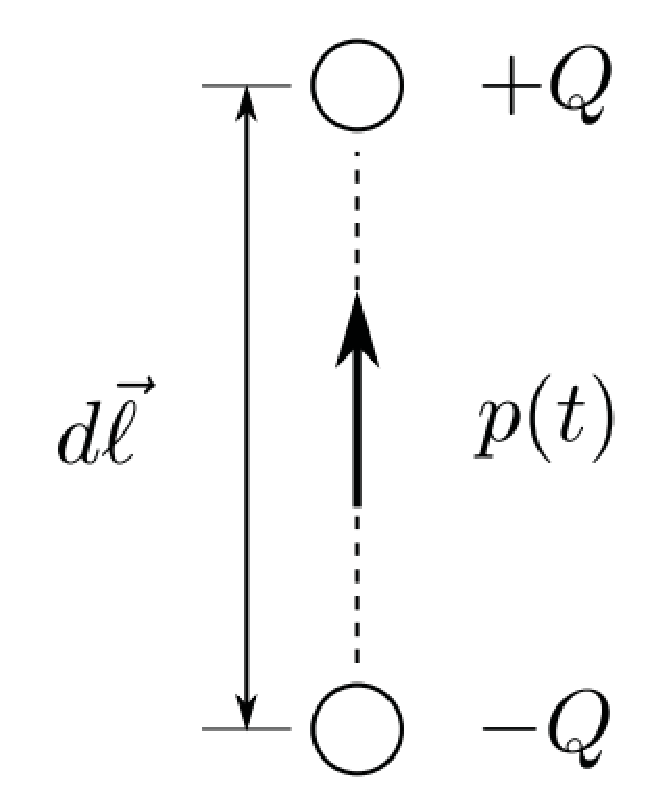
\includegraphics[width=4cm]{content/bilder/HerzDipolEMANTS37.pdf}%
	\caption{Hertzscher Dipol mit dem Dipolmoment \textit{p(t)} \cite{Emant}}
	\label{HerzDipol}
\end{figure}

%\begin{figure}[htbp]
%	\centering
%		\includegraphics[width=8cm]{content/Bilder/Z0_Grafik.png}
%	\caption{Wellenimpdedanz Z0}%
%	\label{Z0_Grafik}
%\end{figure}
Die Ausrichtung der E Feldlinien wechselt bei jeder Schwingung ihre Richtung. Im Nahfeld dominiert das E Feld. Mit wachsendem Abstand sind das E Feld und das H Feld senkrecht aufeinander und in Phase. Dabei können das E und H Feld als ebene Welle betrachtet werden. Die allgemeine Formel für die Feldverteilung lautet \cite{elliott1981antenna}:



\begin{equation}
E_r= \frac{I dl}{2\pi}   e^{-jkR} \left( \frac{n}{R^{2}}  + \frac{1}{j\omega \epsilon R^{3}}\right) cos(\theta)
\end{equation}

\begin{equation}
E_\theta= \frac{I dl}{4\pi}   e^{-jkR} \left( \frac{j\omega \mu}{R}  + \frac{n}{R^{2}}+ \frac{1}{j\omega \epsilon R^{3}}\right) sin(\theta)
\end{equation}

\begin{equation}
H_\phi= \frac{I dl}{4\pi}   e^{-jkR} \left( \frac{jk}{R}  + \frac{n}{R^{2}}\right) sin(\theta)
\end{equation}

Mit wachsendem Abstand können einige Terme vernachlässigt werden. Alle Terme in denen der Abstand R in höherer Potenz vorkommt, werden vereinfacht zu Null. Für das Fernfeld ergeben sich die folgenden Beschreibungen:


\begin{equation}
E_r= 0
\end{equation}

\begin{equation}
E_\theta= \frac{I dl}{4\pi}   e^{-jkR} \left( \frac{j\omega \mu}{R}  \right) sin(\theta)
\end{equation}

\begin{equation}
H_\phi= \frac{I dl}{4\pi}   e^{-jkR} \left( \frac{jk}{R} \right) sin(\theta)
\end{equation}

%Die Terme mit R in der zweiten oder dritten Potenz fallen für das Fernfeld weg. Da im Fernfeld der Radius R so gross ist, dass diese Terme vernachlässig werden. 
%Das Fernfeld kann wie folgt beschrieben werden:
%
%Formel:
%
%Die beiden elementaren Strahler können nicht technisch realisiert werden, aber sie sind sehr wichtig für das Verhalten von realen Antennen. Denn wenn reale Antennen verein-facht werden oder wenn sehr kleine Teilstücke von realen Antennen betrachtet werden, so verhalten sie sich oft wie die elementaren Dipole. 
%
%Die Dipolantenne und die Rahmen Antenne sind den beiden Elementaren Strahleren nachempfunden und sollen im nächsten Abschnitt genauer betrachtet werden.

%%%%%%%%%%%%%%%%%%%%%%%%%%%%%%%%%%%
\begin{figure}[h]
\begin{center}
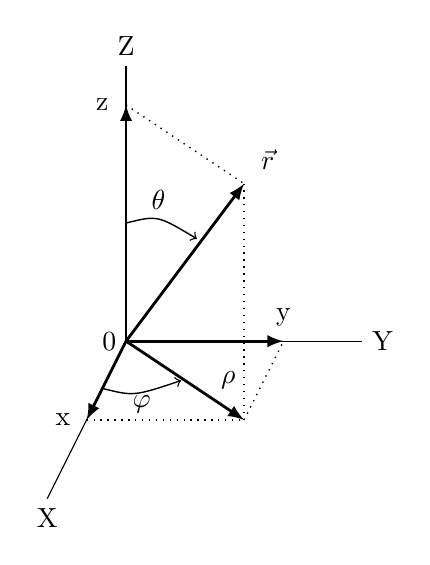
\begin{tikzpicture}
	\draw (4,4) -- (3,2) node[below] {X};%Fadenkreuz x
	\draw (4,4) node[left] {0} -- (7,4)node [right] {Y};%Fadenkreuz y
	\draw (4,4) -- (4,7.5) node[above] {Z};%Fadenkreuz z
	
	\draw[line width=1pt, ->, >=latex](4, 4)  -- (3.5, 3) node at (3.2, 3) {x};
	\draw[line width=1pt, ->, >=latex](4, 4)  -- (6, 4) node at (6, 4.3) {y};
	\draw[line width=1pt, ->, >=latex](4, 4)  -- (4, 7) node at (3.7, 7) {z};
	
	\draw[line width=0.5pt, style=dotted](3.5, 3) -- (5.5, 3);%Projektion y Rcihtung
	\draw[line width=0.5pt, style=dotted](5.5, 3) -- (6, 4);%Projektion x Rcihtung
	
	\draw[line width=1pt, ->, >=latex](4, 4)  -- (5.5, 3) node at (5.3, 3.5) {$\rho$};
	
	\draw[line width=1pt, ->, >=latex](4, 4)  -- (5.5, 6) node at (5.8, 6.3) {$\vec{r}$};
	
	\draw[line width=0.5pt, style=dotted](5.5, 3) -- (5.5, 6);%Projektion p zu \vec{r}
	\draw[line width=0.5pt, style=dotted](4, 7) -- (5.5, 6);%Projektion von z zur \vec{r}
	
	\coordinate (A) at (4, 5.5);
	\coordinate (B) at (4.9, 5.3);
	\coordinate (a) at (4.4, 5.6);
	\draw[line width=0.5pt, cap=round,->](A) .. controls (a) .. node[above] {$\theta$} (B);
	
	\coordinate (C) at (3.7, 3.4);
	\coordinate (D) at (4.7, 3.5);
	\coordinate (c) at (4.1, 3.3);
	\draw[line width=0.5pt, cap=round,->](C) .. controls (c) .. (D) node at (4.2, 3.2){$\varphi$};
\end{tikzpicture}
\end{center}
	\caption{Feldvektor}
	\label{FerdVektor}
\end{figure}

%%%%%%%%%%%%%%%%%%%%%%%%%%%%%%%%%%%%%%%%%%%%%%%%%%%%%%%%%%%%%%%%%%%

%%%%%%%%%%%%%%%%%%%%%%%%%%%%%%%%%%%%%%%%%%%%%%%%%%%%%%%%%%%%%%%%%%%
%\begin{figure}[h]
%\begin{center}
%\begin{tikzpicture}
%	\draw (4,4) -- (3,2)node at (3, 1.7) {X};%Fadenkreuz x
%	\draw (4,4) node[left] {0}-- (7,4)node at (7.3, 4) {Y};%Fadenkreuz y
%	\draw (4,4) -- (4,7.5)node at (3.7, 7.8) {Z};%Fadenkreuz z
%	
%	\draw[line width=1pt, ->, >=latex](4, 4)  -- (3.5, 3) node at (3.2, 3) {x};
%	\draw[line width=1pt, ->, >=latex](4, 4)  -- (6, 4) node at (6, 4.3) {y};
%	\draw[line width=1pt, ->, >=latex](4, 4)  -- (4, 7) node at (3.7, 7) {z};
%	
%	\draw[line width=0.5pt, style=dotted](3.5, 3) -- (5.5, 3);%Projektion y Rcihtung
%	\draw[line width=0.5pt, style=dotted](5.5, 3) -- (6, 4);%Projektion x Rcihtung
%	
%	\draw[line width=1pt, ->, >=latex](4, 4)  -- (5.5, 3) node at (5.3, 3.5) {$\rho$};
%	
%	\draw[line width=1pt, ->, >=latex](4, 4)  -- (5.5, 6) node at (5.5, 6.3) {$\vec{r}$};
%	
%	\draw[line width=0.5pt, style=dotted](5.5, 3) -- (5.5, 6);%Projektion p zu \vec{r}
%	\draw[line width=0.5pt, style=dotted](4, 7) -- (5.5, 6);%Projektion von z zur \vec{r}
%	
%	\coordinate (A) at (4, 5.5);
%	\coordinate (B) at (4.9, 5.3);
%	\coordinate (a) at (4.4, 5.6);
%	\draw[line width=0.5pt, cap=round,->](A) .. controls (a) .. (B) node at (4.4, 5.8){$\theta$};
%	
%	\coordinate (C) at (3.7, 3.4);
%	\coordinate (D) at (4.7, 3.5);
%	\coordinate (c) at (4.1, 3.3);
%	\draw[line width=0.5pt, cap=round,->](C) .. controls (c) .. (D) node at (4.2, 3.2){$\varphi$};
%	
%	%Einheitsvektoren
%	\draw[line width=1pt, ->, >=latex](5.5, 6)  -- (6.1, 6.8) node at (6.5, 7) {$\vec{E_{r}}\vec{e}$};
%	\draw[line width=1pt, ->, >=latex](5.5, 6)  -- (6.1, 5.6) node at (6.5, 5.4) {$\vec{E_{\theta}}\vec{e}$};
%	\draw[line width=1pt, ->, >=latex](5.5, 6)  -- (6.1, 6.3) node at (6.5, 6.1) {$\vec{H_{\varphi}}  \vec{e}$};
%	
%	%Antenne dipol
%	\draw[line width=3pt] (4,4.1) -- (4,5.2);
%	\draw[line width=3pt] (4,3.9) -- (4,2.8);
%\end{tikzpicture}
%\end{center}
%\caption{Dipolantanne mit Feldvektor und Einheitsvektoren}
%\label{DipolEFerdVektor}
%\end{figure}
%%%%%%%%%%%%%%%%%%%%%%%%%%%%%%%%%%%%%%%%%%%%%%%%%%%%%%%%%%%%%%%%%%%

\subsection{Fitzgeraldscher Dipol }\label{sec:FitzgeraldescherDipol}
Eine unendlich dünne Leiterschleife, die auf der ganzen Länge dieselbe Stromverteilung besitzt, wird Fitzgeraldscher Dipol genannt. Dieser Dipol ist das Gegenstück zum Hertzschen Dipol und stellt somit den zweiten der beiden elementaren Strahler dar. Die Leiterschleife ist oft in der xy Ebene angeordnet. Da der Strom oszilliert ist er als \textit{i(t)} gekennzeichnet. Der Strom \textit{i(t)} führt in einem Kreis im Abstand a um das Zentrum. Im Zentrum bildet sich ein magnetisches, zeitabhängiges Moment \textit{m(t)}.
\begin{figure}[!htb]
	\centering
	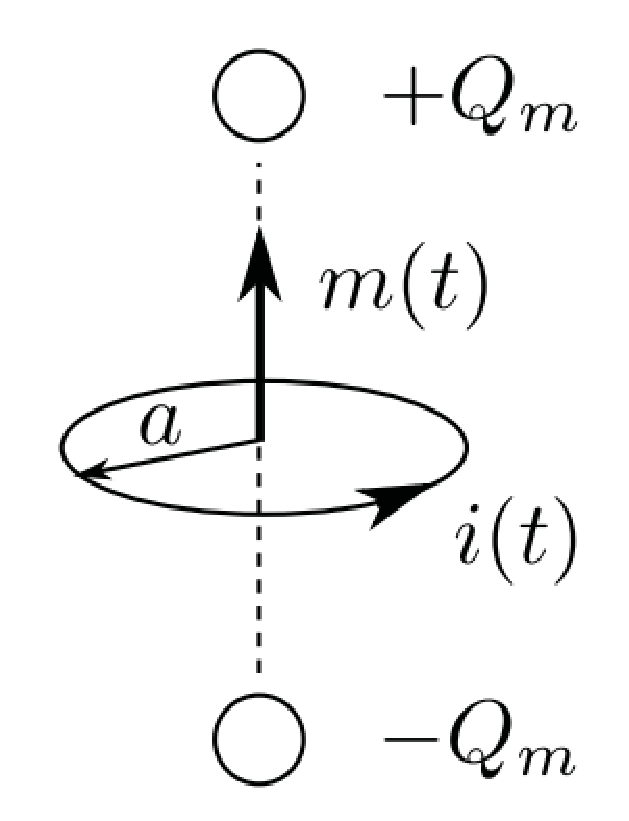
\includegraphics[width=4cm]{content/bilder/Fitzgerald_Dipol_EMANT_S37.pdf}%
	\caption{Fitzgeraldscher Dipol \cite{Emant}}
	\label{FitzDipol}
\end{figure}
Wenn der Hertzsche Dipol eine E Feld Antenne genannt wird, so ist der Fitzgeraldsche Dipol eine H Feld Antenne. Das Nahfeld des Fitzgeraldschen Dipols wird wie folgt beschrieben\cite{elliott1981antenna}:
\todo{fitz Dipol Bild neu Zeichen}

\begin{equation}
H_r= \frac{I S}{2\pi}   e^{-jkR} \left( \frac{jk}{R^{2}}  + \frac{1}{R^{3}} \right) cos(\theta)
\end{equation}

\begin{equation}
H_\theta= \frac{I S}{4\pi}   e^{-jkR} \left(- \frac{k^{2}}{R}  + \frac{jk}{R^{2}}+ \frac{1}{R^{3}} \right) sin(\theta)
\end{equation}

\begin{equation}
E_\phi= \frac{I S}{4\pi}   e^{-jkR} \left( \frac{k^{2}}{R}  - \frac{jk}{R^{2}} \right) sin(\theta)
\end{equation}

Das zeitabhängige magnetische Moment \textit{m(t)} ergibt sich durch die Multiplikation der durch die Schleife aufgespannten Fläche $a^{2}\pi=S$ und dem konstanten Schleifenstrom $I$ der auf der ganzen Schleife denselben Wert $I$ hat. Dank der Annahme des konstanten Strom kann wie in Gleichung \ref{eq:magnetischesMoment} das magnetische Moment berechnet werden \cite{Harrington-TimeHarmonic}. 
\begin{equation}\label{eq:magnetischesMoment}
Ia^{2}\pi=IS=m
\end{equation}

Die Terme mit R in der zweiten oder dritten Potenz fallen für das Fernfeld weg. Da im Fernfeld der Radius R so gross ist, können diese  Terme vernachlässigt werden. 
Das Fernfeld kann wie folgt beschrieben werden:


Formel:
\begin{equation}
H_r= 0
\end{equation}

\begin{equation}
H_\theta= \frac{I S}{4\pi}   e^{-jkR} \left(- \frac{k^{2}}{R}   \right) sin(\theta)
\end{equation}

\begin{equation}
E_\phi= \frac{I S}{4\pi}   e^{-jkR} \left( \frac{k^{2}}{R}   \right) sin(\theta)
\end{equation}

Die beiden elementaren Strahler können nicht technisch  realisiert werden, aber sie sind sehr wichtig für das Verhalten von realen Antennen. Wenn reale Antennen vereinfacht werden oder wenn sehr kleine Teilstücke von realen Antennen betrachtet werden,  verhalten sie sich  wie die elementaren Dipole. \\

Die Dipolantenne und die Rahmenantenne sind den beiden elementaren Strahlern nachempfunden und sollen im nächsten Abschnitt genauer betrachtet werden.

%%%%%%%%%%%%%%%%%%%%%%%%%%%%%%%%%%%%%%%%%%%%%%%%%%%%%%%%%%%%%%%%%%%
\begin{figure}[h]
\begin{center}
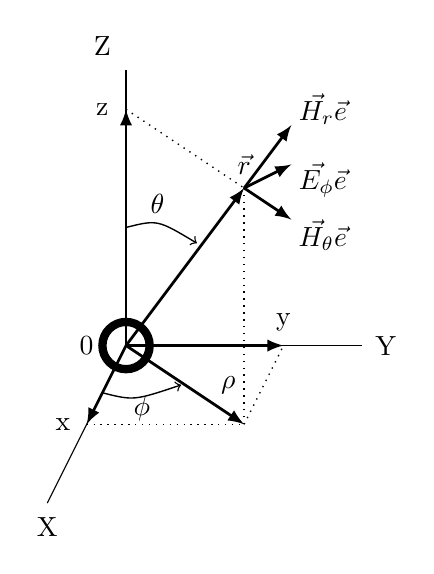
\begin{tikzpicture}
	\draw (4,4) -- (3,2)node at (3, 1.7) {X};%Fadenkreuz x
	\draw (4,4) node at(3.5,4) {0} -- (7,4)node at (7.3, 4) {Y};%Fadenkreuz y
	\draw (4,4) -- (4,7.5)node at (3.7, 7.8) {Z};%Fadenkreuz z
	
	\draw[line width=1pt, ->, >=latex](4, 4)  -- (3.5, 3) node at (3.2, 3) {x};
	\draw[line width=1pt, ->, >=latex](4, 4)  -- (6, 4) node at (6, 4.3) {y};
	\draw[line width=1pt, ->, >=latex](4, 4)  -- (4, 7) node at (3.7, 7) {z};
	
	\draw[line width=0.5pt, style=dotted](3.5, 3) -- (5.5, 3);%Projektion y Rcihtung
	\draw[line width=0.5pt, style=dotted](5.5, 3) -- (6, 4);%Projektion x Rcihtung
	
	\draw[line width=1pt, ->, >=latex](4, 4)  -- (5.5, 3) node at (5.3, 3.5) {$\rho$};
	
	\draw[line width=1pt, ->, >=latex](4, 4)  -- (5.5, 6) node at (5.5, 6.3) {$\vec{r}$};
	
	\draw[line width=0.5pt, style=dotted](5.5, 3) -- (5.5, 6);%Projektion p zu \vec{r}
	\draw[line width=0.5pt, style=dotted](4, 7) -- (5.5, 6);%Projektion von z zur \vec{r}
	
	\coordinate (A) at (4, 5.5);
	\coordinate (B) at (4.9, 5.3);
	\coordinate (a) at (4.4, 5.6);
	\draw[line width=0.5pt, cap=round,->](A) .. controls (a) .. (B) node at (4.4, 5.8){$\theta$};
	
	\coordinate (C) at (3.7, 3.4);
	\coordinate (D) at (4.7, 3.5);
	\coordinate (c) at (4.1, 3.3);
	\draw[line width=0.5pt, cap=round,->](C) .. controls (c) .. (D) node at (4.2, 3.2){$\phi$};
	
	%Einheitsvektoren
	\draw[line width=1pt, ->, >=latex](5.5, 6)  -- (6.1, 6.8) node at (6.5, 7) {$\vec{H_{r}}\vec{e}$};
	\draw[line width=1pt, ->, >=latex](5.5, 6)  -- (6.1, 5.6) node at (6.5, 5.4) {$\vec{H_{\theta}}\vec{e}$};
	\draw[line width=1pt, ->, >=latex](5.5, 6)  -- (6.1, 6.3) node at (6.5, 6.1) {$\vec{E_{\phi}}  \vec{e}$};
	
	%Antenne Loop
\draw[line width=3pt](4, 4) circle (0.3);
\end{tikzpicture}
\end{center}
\caption{Loop Antenne mit Feldvektor und Einheitsvektoren}
\label{LoopFerdVektor}
\end{figure}
%%%%%%%%%%%%%%%%%%%%%%%%%%%%%%%%%%%%%%%%%%%%%%%%%%%%%%%%%%%%%%%%%%%

\subsection{Die Dipol Antenne}\label{sec:DipolAntenne}
Der zentral gespeiste Dipol besteht meistens aus zwei runden Leiterstäben mit dem Durchmesser $d$ und der Länge $l$. Die beidne Stäbe haben eine gesammt Länge von $2l$. Die  Stäbe liegen so aneinander, dass in der Mitte der beiden Stäbe eine kleine Lücke entsteht. Die gesamte Länge der beiden Stäbe ist viel grösser als  der Durchmesser $d$. Wird eine Spannung  in der Lücke zwischen den beiden Stäben angelegt, kommt es zu einer Stromverteilung über die gesamte Länge der  Stäbe. Oft wird die Spannung mit einer Zweidrahtleitung,  diese wird enlisch \textit{Transmission Line} genannt, zwischen den Leiterstäben angebracht. Die anschliessende Stromverteilung der beiden runden Leiterstäbe liefert den Ursprung der Wellenausbreitung. In erster Näherung kann die sich von der Speisestelle ausbreitende Welle als richtungsunabhängige Kugelwelle betrachtet werden \cite{elliott1981antenna}.
%E^j(wt-kr)/4pimu^-1 r
%Elliot Seite 29 Nr1.93
\begin{equation}
\frac{e^{j(\omega t-kr)}}{4\pi \mu_{0}^{-1}r}
\end{equation}

%%%%%%%%%%%%%%%%%%%%%%%%%%%%%%%%%%%%%%%%%%%%%%%%%%%%%%%%%%%%%%%%%%%
\begin{figure}[!htb]
	\centering
	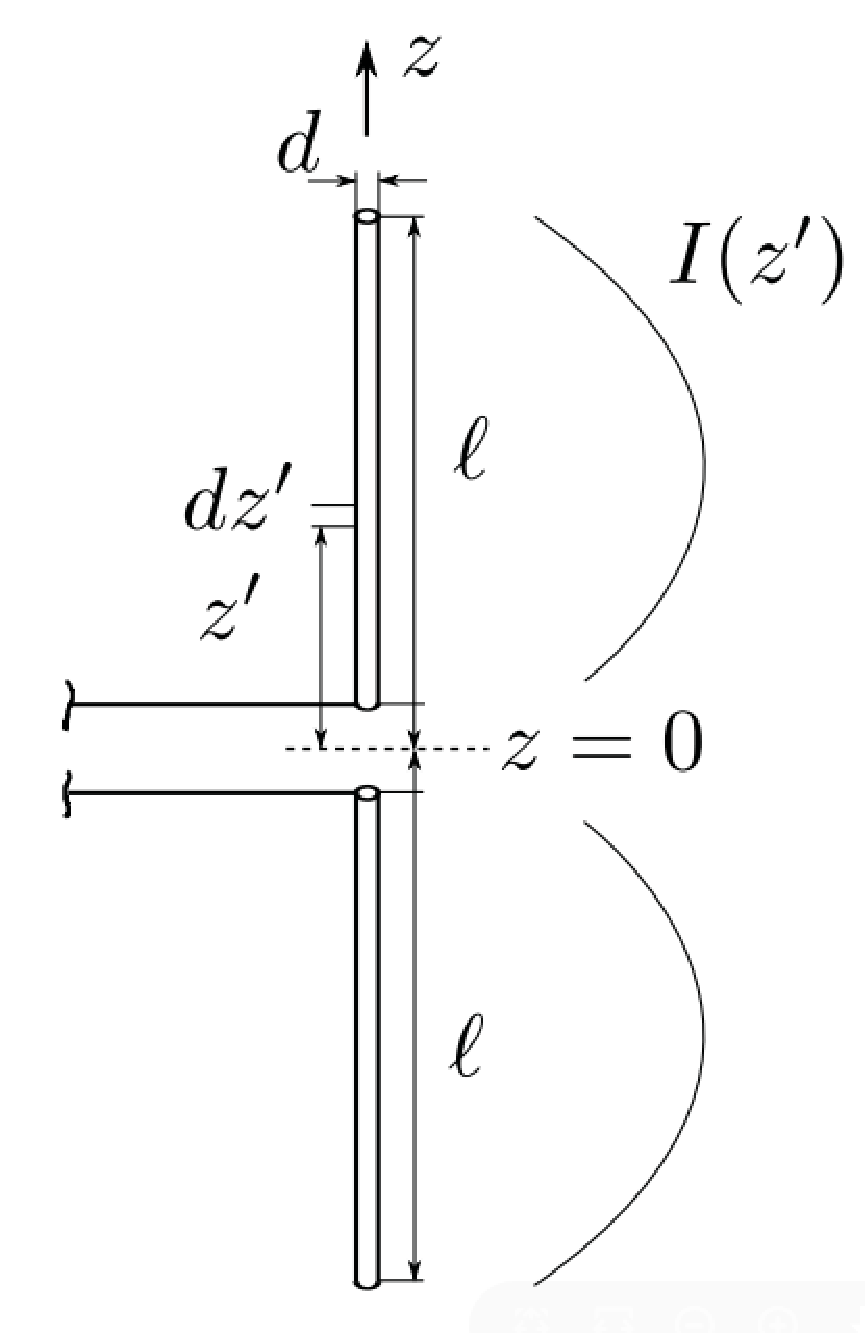
\includegraphics[width=4cm]{content/bilder/Dipol_EMANT_S42.pdf}%
	\caption{Dipol Antenne mit Stromverteilung \cite{Tekom}}
	\label{FitzDipol}
\end{figure}
%%%%%%%%%%%%%%%%%%%%%%%%%%%%%%%%%%%%%%%%%%%%%%%%%%%%%%%%%%%%%%%%%%%

Die Stromausbreitung in der Dipol Stabantenne entspricht der Stromverteilung einer am Ende offenen Zweidrahtleitung. Das offene Ende der Leitung führt zu einer Reflexion der zuführenden Welle in die umgekehrte Richtung und somit zu einer stehenden Welle in der Leitung. Stromführende Elemente, die nahe beieinander liegen, deren Amplituden gleich aber gegenläufig sind, strahlen nur gering. Dies sind Eigenschaften einer guten Zweidrahtleitung.
Als Näherung für die Stromverteilung soll folgendes gelten \cite{elliott1981antenna}:
\begin{equation}
I(x,t) =I_{m}sin([k(l-x)])e^{j\omega t}
\end{equation}
%Elliot Seite 59 Formel 2.1

Bei einem Dipol mit dem Durchmesser $d<<\lambda$ wird dieser zu einem dünnen Stromfaden. Und die Stromdichte im Leiter kann \textbf{J}\textit{d}\textbf{\textbf{V}} mit \textbf{I}\textit{d}\textbf{\textbf{l}} als Stromelement ersetzt werden. Die Summe der Elementardipole kann dann als Quelle betrachtet werden \cite{elliott1981antenna}.\\

\begin{equation}
I_{m}sin(k(l-dz))
\end{equation}
%Elliot Seite 61 Formel 2.2
Die Gewichtungsfunktion dieser Summe von Elementardipolen die alle in der z Achse liegen ist:\\
$a(\phi)= 0$
jedoch die Gewichtungsfunktion in $\theta$ Richtung:
\begin{equation}\label{eq:Gewichtungsfunktion}
a_{\theta}(\theta)=- \frac{2I_{m}}{k sin(\theta)} \lbrack cos(kl cos(\theta)) - cos(kl) \rbrack
\end{equation}
%Elliot Formel 2.6 oder Joss EMANT 122.

Es sollen zwei Fälle genauer betrachtet werden.
\begin{itemize}
\item der Halbwellendipol mit 2l= $\lambda/2$
\item der kurze Dipol mit 2l$<<\lambda$
\end{itemize}
\subsubsection{Der Halbwellendipol}
Der $\lambda/2$ Dipol ist eine der wichtigsten Antennen. Über die Gewichtungsfunktion in Formel \ref{eq:Gewichtungsfunktion} lässt sich auf das Fernfeldverhalten schliessen \cite{elliott1981antenna}.
\todo{Gewichtungsfunktion Nummer}
\begin{equation}
E_{\theta}=j60I_{m} \frac{e^{j(\omega t - kr)}}{r} \lbrack \frac{cos\lbrack  (\pi/2) cos(\theta)\rbrack}{sin(\theta)} \rbrack
\end{equation}
\begin{equation}
H_{\phi}=j \frac{I_{m}}{2\pi} \frac{e^{j(\omega t - kr)}}{r} \lbrack \frac{cos\lbrack  (\pi/2) cos(\theta)\rbrack}{sin(\theta)} \rbrack
\end{equation}
%E(theta)= Ellito 2.8
%E(phi) = Ellito 2.9

Die Feldverteilung kann in der  Zweidimensionalen Polar Form oder in einer Dreidimensionalen Feldverteilung dargestellt werden.
Die nachfolgende Grafik zeigt eine E Feldverteilung als Schnitt durch die xz Ebene.\\
%!!!!Wichtig!!!!!Bild aus Matlab importieren\\
\todo{Matlab Bild der Feldausbreitung}

%%%%%%%%%%%%%%%%%%%%%%%%%%%%%%%%%%%%%%%%%%%%%%%%%%%%%%%%%%%%%%%%%%%
\begin{figure}
\begin{center}
\begin{tikzpicture}
	\draw (0,3) node at (0.5,0.5) {xz Ebene} -- (10,3);%Fadenkreuz horizontal
	\draw (5,0) -- (5,6);%Fadenkreuz vertikal
	\draw [line width=1mm] (5,3.2) -- (5,4.5);%upper arm
	\draw [line width=1mm] (5,1.5) -- (5,2.8);%lower arm
	\draw (3,3) circle (2cm);%linker Kreis
	\draw (7,3) circle (2cm);%rechter Kreis

	\node[draw] at (5,6.5) {$\vartheta=0$};
	\node[draw] at (8,5.5) {$E(\vartheta)$};

\end{tikzpicture}
\end{center}
	\caption{Das E Feld einer Dipolantenne in der xz Ebene}
	\label{fig:DipolEFerd}
\end{figure}

%%%%%%%%%%%%%%%%%%%%%%%%%%%%%%%%%%%%%%%%%%%%%%%%%%%%%%%%%%%%%%%%%%%


Dargestellt ist ein $\lambda/2$ Dipol der in z Richtung aufgerichtet ist. Es ist zu erkennen, dass bei $\theta = 0 ^\circ $  und $\theta = 180 ^\circ $ kein elektrisches Feld abgestrahlt wird. Stellt man sich die Grafik als um eine um $\varphi$ von 0 Grad bis 360 Grad rotierende Scheibe vor, so kommt die bekannte Doughnut Form zum Vorschein.

Die von $\vartheta$ und $\varphi$ abhängige Leitung ist gegeben durch \cite{elliott1981antenna}:
%P(theta,phi)= elliot2.10
\begin{equation}
P(\theta,\phi)=\frac{2\eta I_{m}^{2}}{(4\pi r)^{2}}\lbrack \frac{cos^{2}\lbrack (\pi/2) cos(\theta)\rbrack}{sin^{2}(\theta)}\rbrack
\end{equation}

%Durch Lösung des Doppelintegrals 
%Elliot Seite 63
Durch das Auflösen der Doppelintegrale über $\phi$ von 0 bis $\pi$  und $\theta$ von 0 bis $\pi$ erhält man eine nummerische Lösung der Integrale über die gesamte Kugeloberfläche \cite{elliott1981antenna}:
\begin{equation}
P_{rad}=0.609 \frac{\eta I_{m}^{2}}{2\pi}
\end{equation}
%elliot 63 Forlmel 2.11

Wie die obere Grafik \ref{fig:DipolEFerd} zeigt, ist die maximale Feldausbreitung auf der Höhe der Einspeisestelle bei $\theta = 90 ^\circ $ maximal,  denn der  $sin(90 ^\circ ) $ entspricht 1.
Der maximale Richtwert,  aus dem englischen als \textit{directivity} bekannt, erhält man indem die Abgestrahlte Leistung mit einem isotropen Kugelstrahler verglichen wird\cite{elliott1981antenna}.
\begin{equation}
D(peak)=\frac{P(\theta,\phi)(\pi/2)}{P_{rad}/ 4 \pi r^{2}} =1.64
\label{eq:Directivity}
\end{equation}
%Dmax=1.64 nach Ellito 2.12
\todo{dbi Richtfaktor}

Bei $l=\lambda/4 $ ist der Scheitelwert des Antennenstromes beim Einspeisepunkt, dem Zentrum des Dipol bei z= 0, bei $I_{m}$. Somit kann gesagt werden, dass die Zuleitung  die folgende Leistung  liefert:
%Elliot 2.14
\begin{equation}
P=\frac{1}{2} I_{m}^{2}R_{rad}=(0.609)\frac{\eta I_{m}^{2}}{2\pi}
\end{equation}

Der Strahlungswiderstand oder auch $R_{rad}$ genannt kann im Fall des $\lambda /2$ Dipol nummerisch als 73 Ohm bestimmt werden.
\begin{equation}\label{RradDipol}
R_{rad}=\frac{0.609 \eta}{\pi}= 73 Ohm
\end{equation}
\subsubsection{Der kurze Dipol }\label{sec:kurzerDipol}
\todo{Der kurze Dipol etwas beschreiben}
Die Terme $cos(kl*cos(\theta)) $ und $cos(kl)$ aus der Gewichtungsform des $\lambda/2$ Dipol können mit einer Reihe angenähert werden, sofern kl klein ist.
\begin{equation}
a_{\theta}(\theta)=-kl^{2}I_{m}sin(\theta) \lbrack 1- \frac{(kl)^{2}}{12}(1+cos^{2}(\theta))+...\rbrack
\end{equation}
%Ellito 2.15 Seite 64
Der Eingangsstrom eines kurzen Dipols ist gegeben durch:
\begin{equation}
I=I_{m}sin(kl)=I_{m}\lbrack kl - \frac{(kl)^{3}}{3!} +... \rbrack
\end{equation}
%Ellito 2.16
 Für kleine Längen wie 2l = $\lambda/4 $ kann ohne grossen Fehler die Gewichtingsfunktion als 
%Ellito 2.17
\begin{equation}
a_{\theta}(\theta)=-kl^{2}I_{m}sin(\theta)=-Ilsin\theta
\end{equation}
angenommen werden.
Wie beim $\lambda/2$ Dipol findet man bei einem kurzen Dipol ein vertikal polarisiertes E Feld. Das Feld ist etwas breiter, \todo{Öffnungswinkel angeben} jedoch wie beim $\lambda/2$ Dipol doughnutförmig. Die Impedanz des kurzen Dipols ändert sich jedoch drastisch gegenüber dem $\lambda/2$ Dipol. Mit der Impedanz ist auch die winkelabhängige Leistungsdichte wie folgt gegeben:
%Ellito 2.18
\begin{equation}
P(\theta,\phi)=\frac{(kl)^{2}\eta I^{2}}{2(4\pi r)^{2}}sin^{2}\theta
\end{equation}
Die abgestrahlte Leistung eines kurzen Dipols bei dem über die ganze Kugeloberfläche mit dem Radius $r$ integriert wurde, kann mit der Formel \ref{eq:Rrrad} berechnet werden.
%Ellito 2.19
\begin{equation}\label{eq:Rrrad}
R_{rad}=20 \left(\frac{\pi L}{\lambda} \right) ^{2}
\end{equation}



Die aus der abgestrahlten Leistung ergebende maximale Richtwirkung eines kurzen Dipol wird  mit einem isotopen Strahler verglichen. Dies ergibt nach Formel \ref{eq:Directivity} einen Wert für den Richfaktor D von 1.5. Dieser Wert ist nicht viel weniger als bei einem $\lambda/2$ Dipol mit einem D Wert von 1.64.
Der Strahlungswiderstand kann mit der Umformung des $Prad=1/2 I^{2}Rrad$ umgestellt werden. \\
Man findet :
$Rrad=20\left(piL/\lambda\right)^{2}$
%Eliott
\todo{Rrad brauct es nicht}
Dabei wird L als 2l und somit als länge der beiden Dipolarme angenommen.
Wenn ein Dipol sehr kurz wird, zum Beispiel $2l=\lambda/8$, dann wird $R_{rad} = 3 Ohm$. Dieser Wert ist merklich kleiner als   die 73 Ohm   eines $\lambda/2$ Dipol. Der Effekt auf den reaktiven Anteil der Eingangsimpedanz ist noch dramatischer. Für einen endlich dünnen Dipol mit der Dicke d, ist die Reaktanz der Eingangsimpedanz eines $2l=\lambda/2$ Dipols positiv. Die Reaktanz ist wenig unter Null, wenn die Dipollänge  $2l=\lambda/2$ entspricht. Wird der Dipol weiter gekürzt,  sinkt die Reaktanz sehr schnell ins Negative. Wenn  $2l=\lambda/8$ ist,  sind Werte für X grösser als 1000 Ohm kapazitiv keine Seltenheit. 


\subsection{Loop Antenne}\label{sec:LoopAntenneTheorie}

%%%%%%%%%%%%%%%%%%%%%%%%%%%%%%%%%%%%%%%%%%%%%%%%%%%%%%%%%%%%%%%%%%%
\begin{figure}[h]
	\centering
	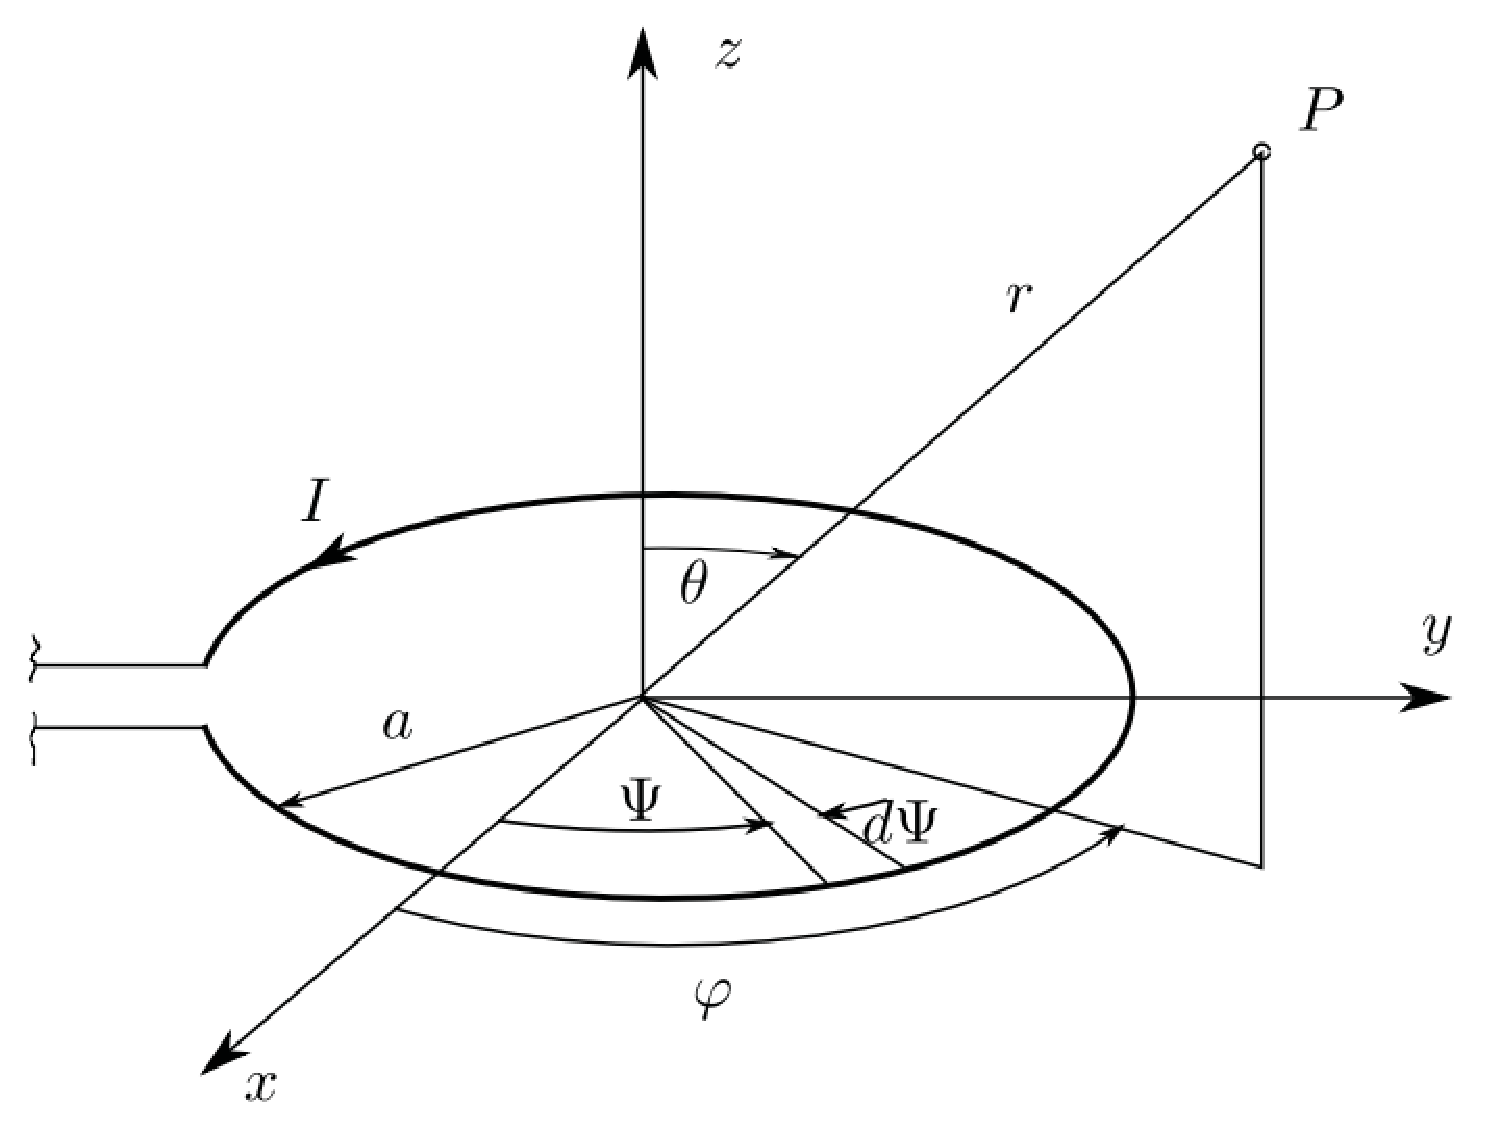
\includegraphics[width=7cm]{content/bilder/Loop_EMANT_S45.pdf}%
	\caption{Loop Antenne}
	\label{LoopAntenne}
\end{figure}
%%%%%%%%%%%%%%%%%%%%%%%%%%%%%%%%%%%%%%%%%%%%%%%%%%%%%%%%%%%%%%%%%%%


Wird eine kurze, kreisförmige Stromschleife mit dem Radius $a<<\lambda$ von einem Strom $Ie^{j\omega t}$ durchflossen,  kann in guter Näherung eine konstante Stromverteilung I entlang der Schlaufe angenommen werden,
Die Koordinaten eines Punktes auf der Stromschleife sind gegeben mit
\begin{eqnarray}
x’ &=&a \cos(\psi)\\
y’ &=&a \sin(\psi)\\
z’ &=&0
\end{eqnarray}


Der Abstand  a entspricht dem Radius  aus dem Zentrum zur Stromschleife. Die Stromschleife ist in  Abbildung \ref{{LoopAntenne}} ersichtlich. Somit kann ein Stromelement auf der Schleife beschrieben werden als:
\begin{equation}
I dl= Ia(- \vec e_{x}sin(\psi)+\vec e_{y}cos(\psi))d\psi
\end{equation}
 
%EMANT Joss Seit 45
Die Stromverteilung führt zu einem Abstrahlen von Elektromagnetischen Wellen.
%Die Gewichtungsfaktoren findet man mit Hilfe von (116 Joss) und (117 Joss) zu
%Emant Joss Seite 46
%Emant Joss Seite 46
Da eine Integration über $2\pi $ einer Kreisfunktion Null ergibt, findet man direkt 
\begin{equation}
a(\theta, \phi) =0
\end{equation}
\todo{Was sthet hier?}
Nimmt man  an, dass $ka$ klein ist, so kann der folgende Term vereinfacht werden.
\begin{equation}
a(\theta)=sin(ka sin(\theta)cos(\psi))=ka sin(\theta)cos(\psi)
\end{equation}
dank der Fereinfachung kann xxxx als geschrieben werden.
\begin{equation}
a(\theta)=j(\pi a^{2}I)(k sin \theta)
\end{equation}
%$a(theta, phi)=j$... oder Ellito 2.31 oder Joss Seite 46.
\todo{neu schreiben Loop}
Das Fernfeld ist  ist  $\varphi$ polarisiert.  Die Leistungsdichte gewinnt man mit 
\todo{Ebenen Loop}
%(Joss 118) 
\begin{equation}
\vec P(\theta,\phi)=\frac{1}{2}Re(\vec E x \vec H^*)
\end{equation}
zu
%Joss EMANT P(theta,phi)=....Ellito 2.32
\begin{equation}
P(\theta)=\frac{(ka)^{4}I{2}\eta}{32r^{2}}sin^{2}\theta
\end{equation}
Im Vergleich mit dem kurzen Dipol erzeugt die kleine Stromschleife ein vergleichbares Richtdiagramm. Das Fernfeld des kurzen Dipols ist jedoch vertikal $\vartheta$ polarisiert. Das bedeutet, dass das Abstrahlverhalten um 90Grad verschoben ist. Integriert man die Leistungsdichte über eine Kugeloberfläche mit dem Radius r  auf und setzt sie der abgegebenen Leistung mit $1/2 I^{2}Rrad $ der zugeführten Zweidrahtleitung gleich, so gewinnt man $R_{rad}$ mit 
\begin{equation}
R_{rad} = 320\pi^{6} (a/\lambda)^{4}\label{eq:RradLoop}
\end{equation}
%ELLITOH 2.33
Beispiel:\\
Wenn $a/\lambda = 0.03$ ist, dann wird der $R_{rad} = 0.25 Ohm$. Als Vergleich mit dem kurzen Dipol mit der Länge $2l=\lambda= 0.06$ führt das zu einem Strahlungswiderstand $R_{rad}$ von 0.7 Ohm.  Der Abstrahlwiderstand $R_{rad}$ einer kleinen Stromschleife kann um den Faktor $n^{2}$ erhöht werden, wenn n die Anzahl der sehr eng aneinander liegenden Wicklungen der Stromschleife sind. 



%%%%%%%%%%%%%%%%%%%%%%%%%%%%%%%%%%%%%%%%%%%%%%%%%%%%%%%%%%%%%%%%%%%

\begin{figure}[h!]
\begin{center}
\begin{tikzpicture}
	\draw (0,3) node at (0.5,0.5) {xz Ebene} -- (10,3);%Fadenkreuz horizontal
	\draw (5,0) -- (5,6);%Fadenkreuz vertikal
	\draw (3,3) circle (2cm);%linker Kreis
	\draw (7,3) circle (2cm);%rechter Kreis
	\draw (4.5,3) circle (0.2cm);%linker kleiner Kreis
	\draw (5.5,3) circle (0.2cm);%rechter kleiner Kreis
	\draw (4.5,3.2) -- (5.5,3.2);%Verbindung horizontal oben
	\draw (4.5,2.8) -- (5.5,2.8);%Verbinung horizontal unten
	\node[draw] at (5,6.5) {$\vartheta=0$};
	\node[draw] at (8,5.5) {$E_{\varphi}(\vartheta)$};

\end{tikzpicture}
\end{center}
\caption{E Feld einer Loop Antenne in der xz Ebene}
\label{DipolEFerd}
\end{figure}
%%%%%%%%%%%%%%%%%%%%%%%%%%%%%%%%%%%%%%%%%%%%%%%%%%%%%%%%%%%%%%%%%%%

\newpage
\subsection{Nah- und Fernfeld}
Antennen sind Wellenwandler. Sie wandeln die ihnen zugeführte elektromagnetische Welle in die elektromagnetische Energie, die sich im Raum um die Antenne ausbreit, um. Die zuführende Welle ist oft an einen elektrischen Leiter gebunden. Dies kann in Form einer Zweidrahtleitung, Leiterbahn auf einer Leiterplatte oder einem Koaxialkabel erfolgen.  Für manche Antennen wird ein Hohlleiter, also Luft als Übertragungsmedium als Zuleitung verwendet . 
Der Antenne kommt die Aufgabe zu, die im Leiter gebundene Welle in eine Raumwelle zu wandeln. Das bedeutet, die leitergebundene Welle wird zu einer Freiraumwelle. Diese füllt den Raum um die Antenne aus. 
Bei einer optimalen Ausführung passt die Antenne den Leitungswiderstand $Z_{L}$ an den Feldwellenwiderstand $Z_{F0}$ von $120\pi = 377 \Omega$ an.
Eine spezielle Ausführung der Antenne als Wellenwandlertyp hängt im wesentlichen vom gewünschten Frequenzbereich und der geforderten Antennencharakteristik ab. Bei einer normalen Freiraumübertagungsstrecke ist die Distanz r zwischen dem Sender und dem Empfänger sehr gross, verglichen mit den Abmessungen der Sendeantennen oder der Freiraumwellenlänge $\lambda_{0}$. Vom Empfangsort scheint die Antennenstrahlung in Bild xx charakterisiert durch den Vektor der elektromagnetischen Leistungsdichte S. 
\todo{Bild xx}
Der Vektor S wird auch Poynting Vektor genannt. Für den Empfänger erscheint es, als ob die empfangene elektromagnetische Strahlung von einem einzigen Punkt ausgeht. Dieser Entstehungspunkt wird Phasenzentrum genannt. Er ist die Quelle der abgestrahlten elektromagnetischen Felder. Wenn diese Voraussetzungen vorliegen, befindet sich der Empfangsort in der Fernfeldregion der Sendeantenne. Die Fernfeldregion wird kurz als Fernfeld bezeichnet. 
Im Fernfeld gelten vereinfachte Beziehungen. Streng genommen liegen nur für die Distanzen von $r->\infty$ reine Fernfeldbedingungen vor. In diesem Fall können die sphärischen Phasenfronten  bereichsweise als eben betrachtet werden. Die am Empfangsort einfallende Welle ist eine ebene Welle für deren elektrische und magnetische Feldstärken die Beziehung \cite{meinke1992taschenbuch}
\todo{Text Bild xx}
\begin{equation}
E/H=120\pi\label{eq:WellenimpedanuE/H}
\end{equation}

gilt. Die Leistungsdichte S ergibt sich, wenn die Feldkomponenten E  und H senkrecht aufeinanderstehen und gleichphasig sind.
\begin{equation}
S=\dfrac{1}{2}EH=\dfrac{1}{2} E^{2}/F_{F0}\label{eq:LeistungsdichteS}
\end{equation}


Die E Feld- und die H Feldkomponente sind dabei Scheitelwerte.
Näherungsweise treten diese Gesetzmässigkeiten auch schon früher bei einem endlichen Abstand r von der Sendeantenne ein. Als Grenzwert für den Fernfeldabstand $r_{2}$ für den Beginn des Fernfeldregion  definiert man in der Praxis für Antennen mit einer grösseren geometrischen Abmessung $D_{0}$ näherungsweise\cite{meinke1992taschenbuch}:
\begin{equation}
r_{2}=\dfrac{2*D_{0}^{2}}{\lambda_{0}} \label{eq:Fernfelddistanz_r2}
\end{equation}

Die maximale Antennenabmessung ist als $D_{0}$ definiert. Für sie gilt $D_{0}>\lambda_{0}$ . Für diese Antennen wird am Empfangsort das Phasenkriterium im Fernfeld eingehalten. Es besagt, dass der Phasenfehler, der durch die Grösse der Antennenabmessungen entsteht, nicht grösser ist als $\lambda_{0}/8$.  Die Gleichung \ref{eq:Fernfelddistanz_r2} berücksichtigt dasselbe Kriterium. Es besagt, dass der Weglängenunterschied $\Delta r$ zwischen zwei am Empfangsort einfallenden Strahlen, von denen der eine vom Antennenmittelpunkt und der andere vom Antennenrand ausgeht, der Bedingung in der Gleichung \ref{eq:Phasenfehler} genügt\cite{meinke1992taschenbuch}.
\begin{equation}
\Delta r\leqq\lambda_{0}/8 \label{eq:Phasenfehler}
\end{equation}
Das Gebiet zwischen dem Sender und dem Empfänger kann in drei Regionen unterteilt werden. Diese sind abhängig von der Distanz $r$ zum Sender. Es können keine klaren Grenzen gezogen werden. Die Übergänge sind fliessend. Zwischen der Sendeantenne und der Fernfeldregion liegt die Nahfeldregion. Diese wird folgend Nahfeld genannt. Das Nahfeld kann in zwei Gebiete unterteilt werden. Es sind dies das Nahfeld und das strahlende Nahfeld. In der  Nahfeldregion, die unmittelbar die Antenne umschliesst, dominieren die reaktiven Feldkomponenten. Die reaktiven Feldkomponeten fallen  mit $r^{3}$ und $r^{2}$ ab.  Je nach Literatur ist die Grenze des Nahfeld zum strahlenden Nahfeld anders definiert. Nach dem Taschenbuch der Hochfrequenztechnik ist dieser Abstand $r_{1}$ erreicht, wenn $r_{1}$ der Formel \ref{eq:Fernfelddistanz_kurzeAntenne} entspricht\cite{meinke1992taschenbuch}.
\todo{bezug zur Formel}

\begin{equation}
R_{1}=0.62\sqrt{\dfrac{D_{0}^{3}}{\lambda_{0}}} \label{eq:Fernfelddistanz_kurzeAntenne}
\end{equation}

Die Beziehungen für die Nahfeldregionen sind von den maximalen Antennenabmessungen abhängig.  Die Definition in Formel \ref{eq:Fernfelddistanz_kurzeAntenne} gilt für Antennen, die als maximale Abmessung $D_{0}>\lambda_{0}$ nicht übersteigt.

Für Dipol und Schleifenantennen, deren Abmessungen wesentlich kleiner als eine Wellenlänge $\lambda_{0}$ sind, erstreckt sich das Nahfeld bis zum  Abstand   $r_{1}=\lambda_{0}/2pi$ von der Antenne.

Bei einer Freiraumübertragungsstrecke, bei der sich die Empfangsantenne im Fernfeld der Sendeantenne im Abstand $r$ befindet, erhält man für die Leistungsdichte am Ort der Empfangsantenne \cite{meinke1992taschenbuch}.

\begin{equation}
S=\dfrac{P_{t}D}{4r^{2}\pi} = \dfrac{P_{t0}G}{4r^{2}\pi}=\dfrac{P_{ei}}{4r^{2}\pi}\label{eq:LeistungsdichteS}
\end{equation}

%Dieser Zusammenhang ist auch im Kapitel yyy in der Gleichung xxx gezeigt.

%
%\begin{figure}
%\begin{center}
%\begin{tikzpicture}
%	\draw[line width=1.5pt](2, 4) circle (0.1) node at (2,3) {Phasenzentrum};
%	\draw (2,1.5) -- (2,0);%Strich nach unten
%	\draw (2,0.3) -- (3,0.3) node at (3.5,0.5) {r};%Strich zum r
%	\draw (4,0.3) -- (5.5,0.3) ;%Strich vom r
%	
%	\draw (2.5,4) -- (3,4);
%	\draw (3.5,4) -- (4,4);
%	\draw (4.5,4) -- (5,4);
%	\draw (5.5,4) -- (6,4);
%	
%	\draw (2.5,4.05) -- (3,4.1);
%	\draw (3.5,4.15) -- (4,4.2);
%	\draw (4.5,4.25) -- (5,4.3);
%	\draw (5.5,4.35) -- (6,4.4);
%	
%	\draw (2.4,4.1) -- (2.9,4.2);
%	\draw (4.4,4.3) -- (4,3.4);
%	\draw (4.2,4.5) -- (5,4.6);
%	\draw (5.1,4.7) -- (6,3.8);
%	
%	\draw (2.5,4.2) -- (3,4.4);
%	\draw (3.5,4.5) -- (4,4.7);
%	\draw (4.5,4.8) -- (5,5);
%	\draw (5.5,5.1) -- (6,5.3);
%%	
%	\draw (2.4,3.95) -- (2.9,3.9);
%	\draw (3.4,3.85) -- (3.9,3.8);
%	\draw (4.4,3.75) -- (4.9,3.7);
%	\draw (5.4,3.65) -- (5.9,3.6);
%
%	\draw (2.3,3.9) -- (3,3.8);
%	\draw (3.3,3.7) -- (4,3.6);
%	\draw (4.3,3.5) -- (5,3.4);
%	\draw (5.3,3.3) -- (6,3.2);
%	
%	\draw (2.5,3.8) -- (3,3.6);
%	\draw (3.5,3.5) -- (4,3.3);
%	\draw (4.5,3.2) -- (5,3);
%	\draw (5.5,2.9) -- (6,2.7);
%
%%	\draw (3,3) circle (2cm);%linker Kreis
%%	\draw (7,3) circle (2cm);%rechter Kreis
%%	\draw (4.5,3) circle (0.2cm);%linker kleiner Kreis
%%	\draw (5.5,3) circle (0.2cm);%rechter kleiner Kreis
%%	\draw (4.5,3.2) -- (5.5,3.2);%Verbindung horizontal oben
%%	\draw (4.5,2.8) -- (5.5,2.8);%Verbinung horizontal unten
%%	\node[draw] at (5,6.5) {$\theta=0$};
%%	\node[draw] at (8,5.5) {$E_{\phi}(\theta)$};
%
%\end{tikzpicture}
%\end{center}
%\caption{Phasenzentrum und Pointingvektor im Antennenfeld}
%\label{fig.Phasenzentrum}
%\end{figure}
%Quelle:Taschenbuch der Hochfrequenztechnik Meineke und Grundach N2
\subsection{Systemansicht}
Die Systemansicht soll einen Überblick über die Bluetooth Verbindung vom Fluginstrument „Connect 1“ zu einem Smartphone geben.
In der nachfolgenden Tabelle werden die Annahmen und  die gegebenen Parameter der Bluetooth Verbindung aufgelistet. Mit der Hilfe des Linkbudgets kann eine Abschätzung des Antennengewinns auf der Empfängerseite hergeleitet werden. Um diese Abschätzung möglich zu machen, werden einige Annahmen getroffen. Zum Beispiel geht man von einer optimalen Anpassung der HF Quelle zur Antenne aus. Weiter wird der Luftraum zwischen Sender und Empfänger als Vakuum angenommen und es hat keine Fremdkörper im Ausbreitungsraum.
Weitere Annahmen sind:
\begin{itemize}
\item Als Sende- und Empfangschip wird beim Empfänger und Sender der CC2541 von TI eingesetzt
\item Freiraum ist Vakuum
\item Keine Hindernisse auf der Übermittlungsstrecke
\item Reserve von 6 dB

\item Der Gewinn der Sendeantenne ist 1
\item Die Sendeleistung ist 0 dBm
\item Die Anschluss- und Verbindungsdämpfung beim Sender und beim Empfänger entsprechen je 0.5 dB
\item -94 dBm Empfangsempfindlichkeit bei 1Mbps und 0.1\% EBR des CC2541 von TI
\end{itemize}

\subsubsection{Linkbudget}
Unter dem Linkbudget versteht man die Summe aller Gewinne und Verluste vom Sender über das Übertragungsmedium bis hin zum Empfänger. Es beschreibt, welcher Signalpegel beim Empfänger nach Abzug aller Verluste ausgehend von der Sendeleistung ankommt. Anhand dieses Wertes und den technischen Angaben des Empfängers kann im voraus die maximal mögliche Datenrate berechnet werden. Wenn die Sendeleitung gesetzlich limitiert ist und die maximale Bit Fehler Rate (EBR) bekannt ist, kann die maximale Distanz oder die maximale Datenrate berechnet werden. Ist die Sendeleistung nicht beschränkt, so kann durch umstellen der Formel die theoretisch erreichbare Sendedistanz ermittelt werden. 
Das Linkbudget kann  nahezu beliebig komplex gestaltet werden und eine  Reihe von weiteren Parametern beinhalten. In der Praxis hat sich für die Berechnung des Linkbudgets bei Richtfunksystemen nach  Formel \ref{eq:LinkBudgetGelichung} bewährt.


\begin{equation}
P_{Rx} = P_{Tx}+L_{Tx}+G_{x}+L_{fs}+L_{Rx}+G_{r}+L_{div}\label{eq:LinkBudgetGelichung}
\end{equation}

Die Formel \ref{eq:LinkBudgetGelichung} wird als Ausgangslage für die Berechnung des minimalen Gewinns der Sendeantenne $G_{x}$ dienen. Da  die minimale Empfängersensitivität aus dem Daten Blatt des  Bluetooth Low Energie Texas Instruments CC2541 Chip bekannt ist, kann der nötige Gewinn der Sendeantenne $G_{x}$ berechnet werden. Der minimale Gewinn ist ein Kriterium welches beim Antennendesign beachtet werden muss.

Der Empfangspegel $P_{Rx}$ in der Fromel \ref{eq:LinkBudgetGelichung}  steht für die am Empfäger resultierende Leitung in dBm.  Die Sendeleistung $P_{Tx}$ in dBm und $L_{Tx}$ steht für jegliche Verluste durch Kabel, Verbinder und Stecker in dB auf der Senderseite. Der Gewinn der Sendeantenne ist als $G_{x}$ angegeben und hat die Einheit dBi. $G_{r}$ steht für den Gewinn (englisch gain) der Empfangsantenne. $L_{fs}$ steht für den Verlust durch die Freiraumdämpfung in dB, $L_{div}$  für diverse weitere Verluste wie zum Beispiel Hindernisse oder für eine System Reserve.  $L_{Rx}$ steht für jegliche Verluste durch Kabel, Verbinder, Stecker in dB von der Empfangsantenne bis zum Empfänger.


Die Freiraumdämpfung $L_{fs}$ soll an dieser Stelle etwas genauer erläutert werden. Unter der Freiraumdämpfung (engl. Free Space Path Loss)  versteht man die Reduzierung der Leistungsdichte bei der Ausbreitung von elektromagnetischen Wellen im freien Raum. Im Vakuum existieren keine Störeinflüsse wie zu Beispiel die Dämpfung durch Luft, andere Gase oder  Hindernisse. Somit wird das Medium als homogen  und Reflexionsfrei angenommen. Anders ausgedrückt, der Pfadverlust beschreibt den Verlust an elektromagnetischer Leistung zwischen einem Sender und Empfänger.
In der Theorie wird von einem isotropen Kugelstrahler ausgegangen, also einem Strahler, der gleichmässig und verlustfrei in alle Richtungen in den Raum abstrahlt. Daraus folgt, dass die abgestrahlte Energie gleichmässig in den Raum verteilt wird und somit an jedem beliebigen Punkt mit gleicher Entfernung zum Strahler identisch ist. So bilden sich Kugeln mit gleicher Leistungsdichte um den Strahler. Je grösser der Abstand zum Strahler wird, desto mehr verteilt sich die Energie auf eine immer grösser werdende Oberfläche. Hierbei ist der Verlust durch die Freiraumdämpfung proportional zu dem Quadrat der Entfernung $R$ zwischen Sender und Empfänger und zu dem Quadrat der verwendeten Frequenz.
\cite{linkbudget}

%%%%%%%%%%%%%%%%%%%%%%%%%%%%%%%%%%%%%%%%%%%%%%%%%%%%%%%%%%
\begin{figure}[h]
\begin{center}
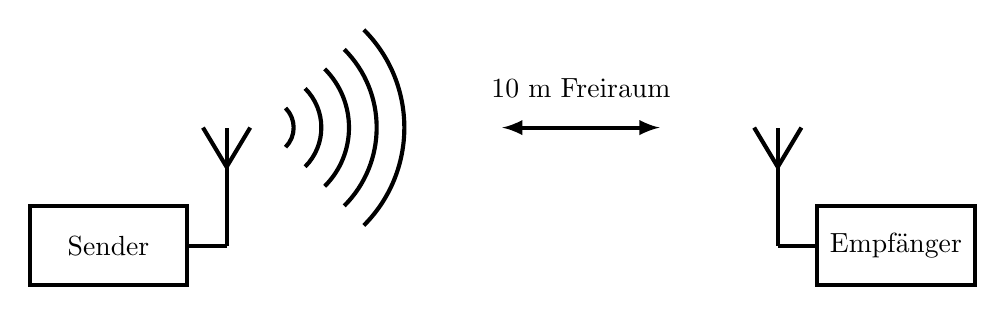
\begin{tikzpicture}
	\draw[line width=1.5pt](0, 0) rectangle (2, 1) node[pos=0.5] {Sender};
	\draw[line width=1.5pt] (2, 0.5) -- (2.5, 0.5);%zuleitung
	\draw[line width=1.5pt] (2.5, 0.5) -- (2.5, 1.5);%Antennenmast
	\draw[line width=1.5pt] (2.5, 1.5) -- (2.2, 2);%Antenne
	\draw[line width=1.5pt] (2.5, 1.5) -- (2.8, 2);
	\draw[line width=1.5pt] (2.5, 1.5) -- (2.5, 2);
	
	\draw[line width=1.5pt, <->, >=latex](6, 2)  -- (8, 2) node at (7, 2.5) {10 m Freiraum};
	
	\draw[line width=1.5pt] (9.5, 0.5) -- (10, 0.5);%zuleitung
	\draw[line width=1.5pt] (9.5, 0.5) -- (9.5, 1.5);%Antennenmast
	\draw[line width=1.5pt] (9.5, 1.5) -- (9.2, 2);%Antenne
	\draw[line width=1.5pt] (9.5, 1.5) -- (9.8, 2);
	\draw[line width=1.5pt] (9.5, 1.5) -- (9.5, 2);
	\draw[line width=1.5pt,decorate,decoration=expanding waves](3, 2) -- (5, 2);
	\draw[line width=1.5pt](10, 0) rectangle (12, 1) node[pos=0.5] {Empfänger};
	%\node[draw,text] at (1,0.5) {Sender};
%	\node[draw,text] at (9,0.5) {Empfenger};
\end{tikzpicture}
\end{center}
\caption{Verbindungs Modell}
\label{fig:LinkModell}
\end{figure}
%%%%%%%%%%%%%%%%%%%%%%%%%%%%%%%%%%%%%%%%%%%%%%%%%%%%%%%%%%%

Die Abbildung \ref{fig:LinkModell} zeigt ein einfaches Verbindungsmodell einer Richtstrahlverbindung. Das in der Tabelle \ref{tab:Linkbudget} aufgezeigte Linkbudget beschreibt eine Übertragung wie in Gleichung \ref{eq:LinkBudgetGelichung} gezeigt wird. Es werden einige Vereinfachungen getroffen. Der Gewinn der Empfangsantenne $G_{r}$  ist als Faktor 1 definiert, das entspricht 0dBi. Es werden keine Polarisationsverluste berücksichtigt. Für die Berechnung der Freiraumdämpfung $L_{fs}$ wird als Übertragungsmedium Vakuum angenommen. Als Sende- und Empfangschip wird der in der \glqq Connect 1\grqq zur Anwendung kommende Texas Instruments CC2541 Chip angenommen.
\begin{eqnarray}
    	d_{0} 	&=& x \\ \label{eq:d0_LinkBudget}
    K		&=& \left(\dfrac{\lambda}{4\pi d_{0}} \right)^{2}G_{x}G_{r} \\ \label{eq:K_LinkBudget}
    P_{Rx} 	&=& P_{Tx}K \left( \dfrac{d_{0}}{D}\right)^{\gamma} \\ \label{eq:Prx_LinkBudget}
    L_{fs} 	&=& \dfrac{P_{Tx}}{P_{Rx}} \\ \label{eq:Freiraumdaempfung}
    L_{fs}(dB) 	&=& 10\log_{10}(L_{fs}) \label{eq:Freiraumdaempfung_dB}
\end{eqnarray}


\begin{table}[h]
  \centering
  \begin{tabular}{l c r} \toprule 
  Komponete                  	& 			&Leistungsbeitrag  \\ \midrule
  Abgegebene Leitung    			&$P_{Tx}$ 	& 0dB       \\
  Übergangsverluste              &$L_{Tx}$	& -3dB       \\
  Gewinn der Sendeantenne    	&$G_{x}$		& zu bestimmen        \\
  Ausbreitungsverluste   		& $F_{LS}$	& -60dB        \\
  Gewinn Empfangsantenne  		& $G_{r}$	& 0dB           \\
  Polarisationsverluste          & 	& 0dB            \\
  Übergangsverluste              & $L_{Rx}$	& -3dB            \\
  Erwartete Leistung am Empfänger & $P_{Rx}$  & -66dBm \cite{CC2541} \\ \midrule
  Systemreserve        			 & $L_{div}$&-6dBm \\ 
  Minimal notwendiges Empfängersignal &$P_{Rx}^{'}$ & -72dB \\ \bottomrule
  \end{tabular}
  \caption{Linkbudget 10m Bluetooth Übertragung}
  \label{tab:Linkbudget}
\end{table}
%%%%%%%%%%%%%%%%%%%%%%%%%%%%
%%%%Quelle&%%%%%%%%%%%
%%%%%%%%%%%%%%%%%%%%%%%%%
\newpage
\subsection{Quelle}
Jedes Antennensystem verfügt über eine Quelle.  Die Quelle liefert an ihrem Ausgang ein hochfrequentes Signal. Der Ausgang kann entweder symmetrisch oder asymmetrisch sein. Die Ausgangsimpedanz von Quellen kann sehr unterschiedlich sein. Oft findet sich am Quellenausgang ein Anpassungsnetzwerk, um die Quellenimpedanz an die Leitungsimpedanz anzupassen. Die in der Hochfrequenztechnik verwendeten Quellen haben oft einen Innenwiderstand von $50\Omega$. Die Abbildung \ref{fig:asymetrischeQuelle} zeigt eine asymmetrische  Hochfrequenzquelle. Einer der beiden Anschlüsse wird als Massenpotential definiert, der andere Anschluss führt das gewünschte Signal. 
\begin{figure}[h]
	\begin{center}
	\begin{tikzpicture}
	\draw[line width=1.5pt](3, 3.5) circle (0.5) node at (3,3.5) {Uq};
	\draw[line width=1.5pt] (3, 5) -- (4.5, 5);
	%\draw[line width=1.5pt] (3, 2) -- (7, 2);
	\draw[line width=1.5pt, -*](3, 2)  -- (7, 2);
	\draw[line width=1.5pt] (3, 2) -- (3, 3);
	\draw[line width=1.5pt] (3, 4) -- (3, 5);
	\draw[line width=1.5pt](4.5, 4.75) rectangle (5.5, 5.25) node at (5, 5.5) {Rq} node at (5, 4.5) {50 Ohm};
	%\draw[line width=1.5pt] (5.5, 5) -- (7, 5);
	\draw[line width=1.5pt, -*](5.5, 5)  -- (7, 5);
	\draw[line width=1.5pt, decorate, decoration=snake](8, 5) -- (9, 5) node at (8.5, 5.5) {Signal der Quelle};
	\draw[line width=1.5pt](2, 1.5) rectangle (6.5, 6) ;%Quellenramen
	\draw[line width=1.5pt] (7, 2) -- (8, 2);%Masse Strich horizontal
	\draw[line width=1.5pt] (8, 2) -- (8, 1.5);%Masse Strich vertikal
	\draw[line width=1pt] (7.5, 1.5) -- (8.5, 1.5);%Masse Strich horizontal kurz
	\draw[line width=1pt] (7.7, 1.3) -- (8.3, 1.3);%Masse Strich horizontal kurz
	\draw[line width=1pt] (7.9, 1.1) -- (8.1, 1.1);%Masse Strich horizontal kurz
	\end{tikzpicture}
	\end{center}
\caption{ESB einer asymetrischen Quelle}
\label{fig:asymetrischeQuelle}
\end{figure}

Symmetrische Quellen haben zwei oder drei Anschlusspunkte. Sie übertragen das HF Signal auf zwei Leitungen. Die Signalform ist um 180$^\circ$ auf den beiden Leitungen zu einander verschoben. Eine symmetrische Quelle ist in der Abbildung \ref{fig:symetrischeQuelle} dargestellt.
\begin{figure}[h]
	\begin{center}
	\begin{tikzpicture}
	\draw[line width=1.5pt](3, 3.5) circle (0.5) node at (3,3.5) {Uq};
	\draw[line width=1.5pt] (3, 5) -- (4.5, 5);
	%\draw[line width=1.5pt] (3, 2) -- (7, 2);
	\draw[line width=1.5pt, -*](3, 2)  -- (8, 2);
	\draw[line width=1.5pt] (3, 2) -- (3, 3);
	\draw[line width=1.5pt] (3, 4) -- (3, 5);
	%\draw[line width=1.5pt](4.5, 4.75) rectangle (5.5, 5.25) node at (5, 5.5) {Rq} node at (5, 4.5) {50 Ohm};
	\draw[line width=1.5pt] (4.5, 4) -- (4.5, 6);%Spliter
	\draw[line width=1.5pt] (4.5, 6) -- (5.5, 6);%Spliter oben
	\draw[line width=1.5pt] (4.5, 4) -- (5.5, 4);%Spliter unten
	\draw[line width=1.5pt] (5.5, 5.5) -- (5.5, 6.5);%Verstärker hinten
	\draw[line width=1.5pt] (5.5, 6.5) -- (6.5, 6);%obenaben
	\draw[line width=1.5pt] (5.5, 5.5) -- (6.5, 6);%untenufen
	\draw[line width=1.5pt] (5.5, 3.5) -- (5.5, 4.5);%Inverter hinten
	\draw[line width=1.5pt] (5.5, 4.5) -- (6.5, 4);%obenaben
	\draw[line width=1.5pt] (5.5, 3.5) -- (6.5, 4);%untenufen
	\draw[line width=1.5pt, -*](6.5, 6)  -- (8, 6);%Siganlpfad oben
	\draw[line width=1.5pt](6.6, 4) circle (0.1);
	\draw[line width=1.5pt, -*](6.7, 4)  -- (8, 4);%Siganlpfad unten
	\draw[line width=1.5pt, decorate, decoration=snake](9, 6) -- (10, 6) node at (9.5, 6.5) {Signal der Quelle};
	\draw[line width=1.5pt, decorate, decoration=snake](9, 4) -- (10, 4) node at (9.5, 4.5) {Signal der Quelle invertiert};
	\draw[line width=1.5pt](2, 1.5) rectangle (7, 7) ;%Quellenramen
	\draw[line width=1.5pt] (8, 2) -- (9, 2);%Masse Strich horizontal
	\draw[line width=1.5pt] (9, 2) -- (9, 1.5);%Masse Strich vertikal
	\draw[line width=1pt] (8.5, 1.5) -- (9.5, 1.5);%Masse Strich horizontal kurz
	\draw[line width=1pt] (8.7, 1.3) -- (9.3, 1.3);%Masse Strich horizontal kurz
	\draw[line width=1pt] (8.9, 1.1) -- (9.1, 1.1);%Masse Strich horizontal kurz
	\end{tikzpicture}
	\end{center}
\caption{ESB einer symetrischen Quelle}
\label{fig:symetrischeQuelle}
\end{figure}
\subsection{Zuleitung}
Darunter versteht man die Verbindung zwischen Quelle und Antenne. Je nach System kommen Zweidrahtleitungen, Koaxialleitungen oder Hohlleiter zum Einsatz. Eine Zweidrahtleitung ist eine symmetrische Verbindung, während ein Koaxialkabel eine asymmetrische Verbindung darstellt.
Weiter Verbindungstypen sind:
\begin{itemize}
\item Drahtverbindung
\item Koaxialkabel
\item Leiterbahn
\item Hohlleiter
\item Glasfaserleiter
\end{itemize}
An dieser Stelle soll genauer auf die elektrische leitergebundene Übertragung eingegangen werden.
Leitungen gehören zu den wichtigsten Übertragungsmedien der Nachrichtentechnik. Sie leiten fast mit Lichtgeschwindigkeit elektromagnetische Wellen vom Sendeort zum Empfangsort.
Bei Gleichstrom und sehr niedrigen Frequenzen kann eine Leitung im allgemeinen als ideal oder mit einem rein ohmischen Verhalten angenommen werden. Man macht keine grossen Fehler, wenn man Signalverläufe am Eingang und am Ausgang als gleich und gleichzeitig ansieht. Kommt aber die physikalische Länge der Leitung in die Grössenordnung der Wellenlänge der Schwingung oder die Anstiegszeit eines Impulses in die Grössenordnung der Ausbreitungsverzögerung, dann kann die Ausgangsspannung völlig anders aussehen als die Eingangsspannung. Die Leitung muss jetzt als Zweitor mit frequenzabhängigen Eigenschaften betrachtet werden.
Ein geeignetes Konzept für das Verständnis ist der Begriff der elektrischen Länge:
\begin{equation}
Elektrische Länge=\dfrac{l}{\lambda}\label{eq:ElektrischeLänge}
\end{equation}

Bei der  Gleichung \ref{eq:ElektrischeLänge} ist $l$ die Länge der Leitung und $\lambda$ gibt die Wellenlänge des Signales auf der Leitung mit der Länge $l$ an. 
			
Zur Analyse, ob eine Leitung strahlt, wird ihre Elektrische Länge betrachtet. \\
Ist die $Elektrische Länge=\dfrac{l}{\lambda} \le \dfrac{1}{20}$  kann die Leitung mit der klassischen Schaltungstheorie behandelt werden. Die Leitung wird meist als verlustlos und reflexionsfrei betrachtet.\\
Ein etwas anders Bild zeigt sich, wenn die $Elektrische Länge=\dfrac{l}{\lambda}>\dfrac{1}{20}$ entspricht. In deisem Fall muss die Leitung als frequeznabäniges Zweitor betrachtet werden. Die Phänomene der elektromagnetischen Wellen werden wirksam. Die Leitungen müssen mit ihren frequenzabhängigen Eigenschaften behandelt werden. 
Geht man von einer idealen Wellenausbreitung aus, bei der keine Verluste vorkommen, so ist die Wellenlänge $\lambda$ mit der Signalfrequenz $f$ und mit der Lichtgeschwindigkeit $c$ wie in Gleichung \ref{eq:WellenlängeMITc} verknüpft.
\begin{equation}
\lambda_{0}=\dfrac{c}{f}\label{eq:WellenlängeMITc}
\end{equation}
Da eine Leitung immer etwas Verlustbehaftet ist, kann die Ausbreitung einer Welle im Leitermedium nie der Lichtgeschwindigkeit $c$ entsprechen. Daher gilt:
\begin{equation}
\lambda=\dfrac{v}{f}\label{eq:WellenlängeMITv}
\end{equation}
Die Signalgeschwindigkeit $v$ dividiert durch die Anzahl Schwingungen pro Sekunde ergibt die Wellenlänge $\lambda$.

Für die Gleichungen \ref{eq:ElektrischeLänge}, \ref{eq:WellenlängeMITc} und \ref{eq:WellenlängeMITv} gilt:
\begin{enumerate}[leftmargin=2cm]
   \item[] l: Leitungslänge [m] 
   \item[] $\lambda$: Wellenlänge  [m] 
   \item[] $f$: Frequenz (Hz) [1/s] 
   \item[] $c$: Lichtgeschwindigkeit  [m/s] 
   \item[] $v$: Geschwindigkeit  [m/s] 
\end{enumerate} 
Besonders vorteilhafte Übertragungseigenschaften hat die längshomogene Leitung. Es handelt sich dabei um eine Leitung, die auf ihrer ganzen Länge einen konstanten Leitungsquerschnitt, gleiches
Leitermaterial, konstanten Leiterabstand und einen gleichförmigen Isolator hat. Gebräuchliche Formen sind die symmetrische Zweidrahtleitung, die verdrillte Zweidrahtleitung, eine Streifenleitung auf
einer Printplatte oder das Koaxialkabel.
\subsubsection{Leitungsmodell}
Um die Zweitoreigenschaften einer längshomogenen Leitung zu ermitteln, wird diese wie in
Abbildung \ref{fig:LeitungsmodellZweitorKette} dargestellt. Diese wird in $n$ gleiche Elementarzweitore unterteilt, wobei $n$ sehr gross sein soll. Dabei wird die Leitung in eine Vielzahl von Zweitoren unterteilt. Es ist von einer Zweitorkette die Rede.
\begin{figure}[h]
	\begin{center}
	\begin{tikzpicture}
	%unten
	\draw[line width=0.5pt, *-*](2, 2)  -- (3.5, 2);
	\draw[line width=0.5pt, -*](3.5, 2)  -- (5, 2);
	\draw[line width=0.5pt, -*](5, 2)  -- (6.5, 2) ;
	\draw[line width=0.5pt, -*](6.5, 2)  -- (8, 2);
	\draw[line width=0.5pt, -*](8, 2)  -- (9.5, 2);
	%oben
	\draw[line width=0.5pt, *-*](2, 3.5)  -- (3.5, 3.5);
	\draw[line width=0.5pt, -*](3.5, 3.5)  -- (5, 3.5);
	\draw[line width=0.5pt, -*](5, 3.5)  -- (6.5, 3.5) node at (5.75,4) {$\Delta z$};
	\draw[line width=0.5pt, -*](6.5, 3.5)  -- (8, 3.5);
	\draw[line width=0.5pt, -*](8, 3.5)  -- (9.5, 3.5)node at (8.75,4) {$n$};
	\draw[line width=1.5pt, ->, >=latex](2, 3.2) -- (2, 2.3) node at (1.5,2.75) {$\underline{U_{1}}$};
	\draw[line width=1.5pt, ->, >=latex](9.5, 3.2) -- (9.5, 2.3) node at (10,2.75) {$\underline{U_{2}}$};
	%vertikal gepunktete linien
	\draw[line width=0.5pt, style=dashed](3.4, 2) -- (3.4, 3.5);%vertikal gepunktete Linie
	\draw[line width=0.5pt, style= dashed](4.9, 2) -- (4.9, 3.5);%vertikal gepunktete Linie
	\draw[line width=0.5pt, style= dashed](6.4, 2) -- (6.4, 3.5);%vertikal gepunktete Linie
	\draw[line width=0.5pt, style=dashed](7.9, 2) -- (7.9, 3.5);%vertikal gepunktete Linie
	\end{tikzpicture}
	\end{center}
\caption{Leitungsmodell eine Kette von Zweitoren}
\label{fig:LeitungsmodellZweitorKette}
\end{figure}
Wie in der Abbildung \ref{fig:LeitungsmodellZweitorKette} gezeigt ist, kann die Leiterlänge durch $n$ geteilt werden. Da $n$ sehr gross ist, ergeben sich n+1 $\Delta z$ lange Leiterstücke. Betrachtet man ein kurzes Leitungsstück mit der Länge $\Delta z = 1/n$, so ist von der Elektrotechnik  bekannt, dass beim Einschalten einer Signalquelle sich auf der Leitung ein Strom $i(t)$ einstellt. \\Die Folge davon ist ein magnetisches Feld radial um die Leitung. Der magnetische Fluss ergibt sich mit der Abschnittsinduktivität zu $\phi = i  \Delta L$. \\
Das einschalten der Quelle führt weiter zu einer  Spannung zwischen den Leitern. Die Folge davon ist ein elektrisches Feld und eine Oberflächenladung $Q = u  \Delta C$ auf den Leitern \cite{Emant}.

\begin{figure}[!htb]
	\centering
	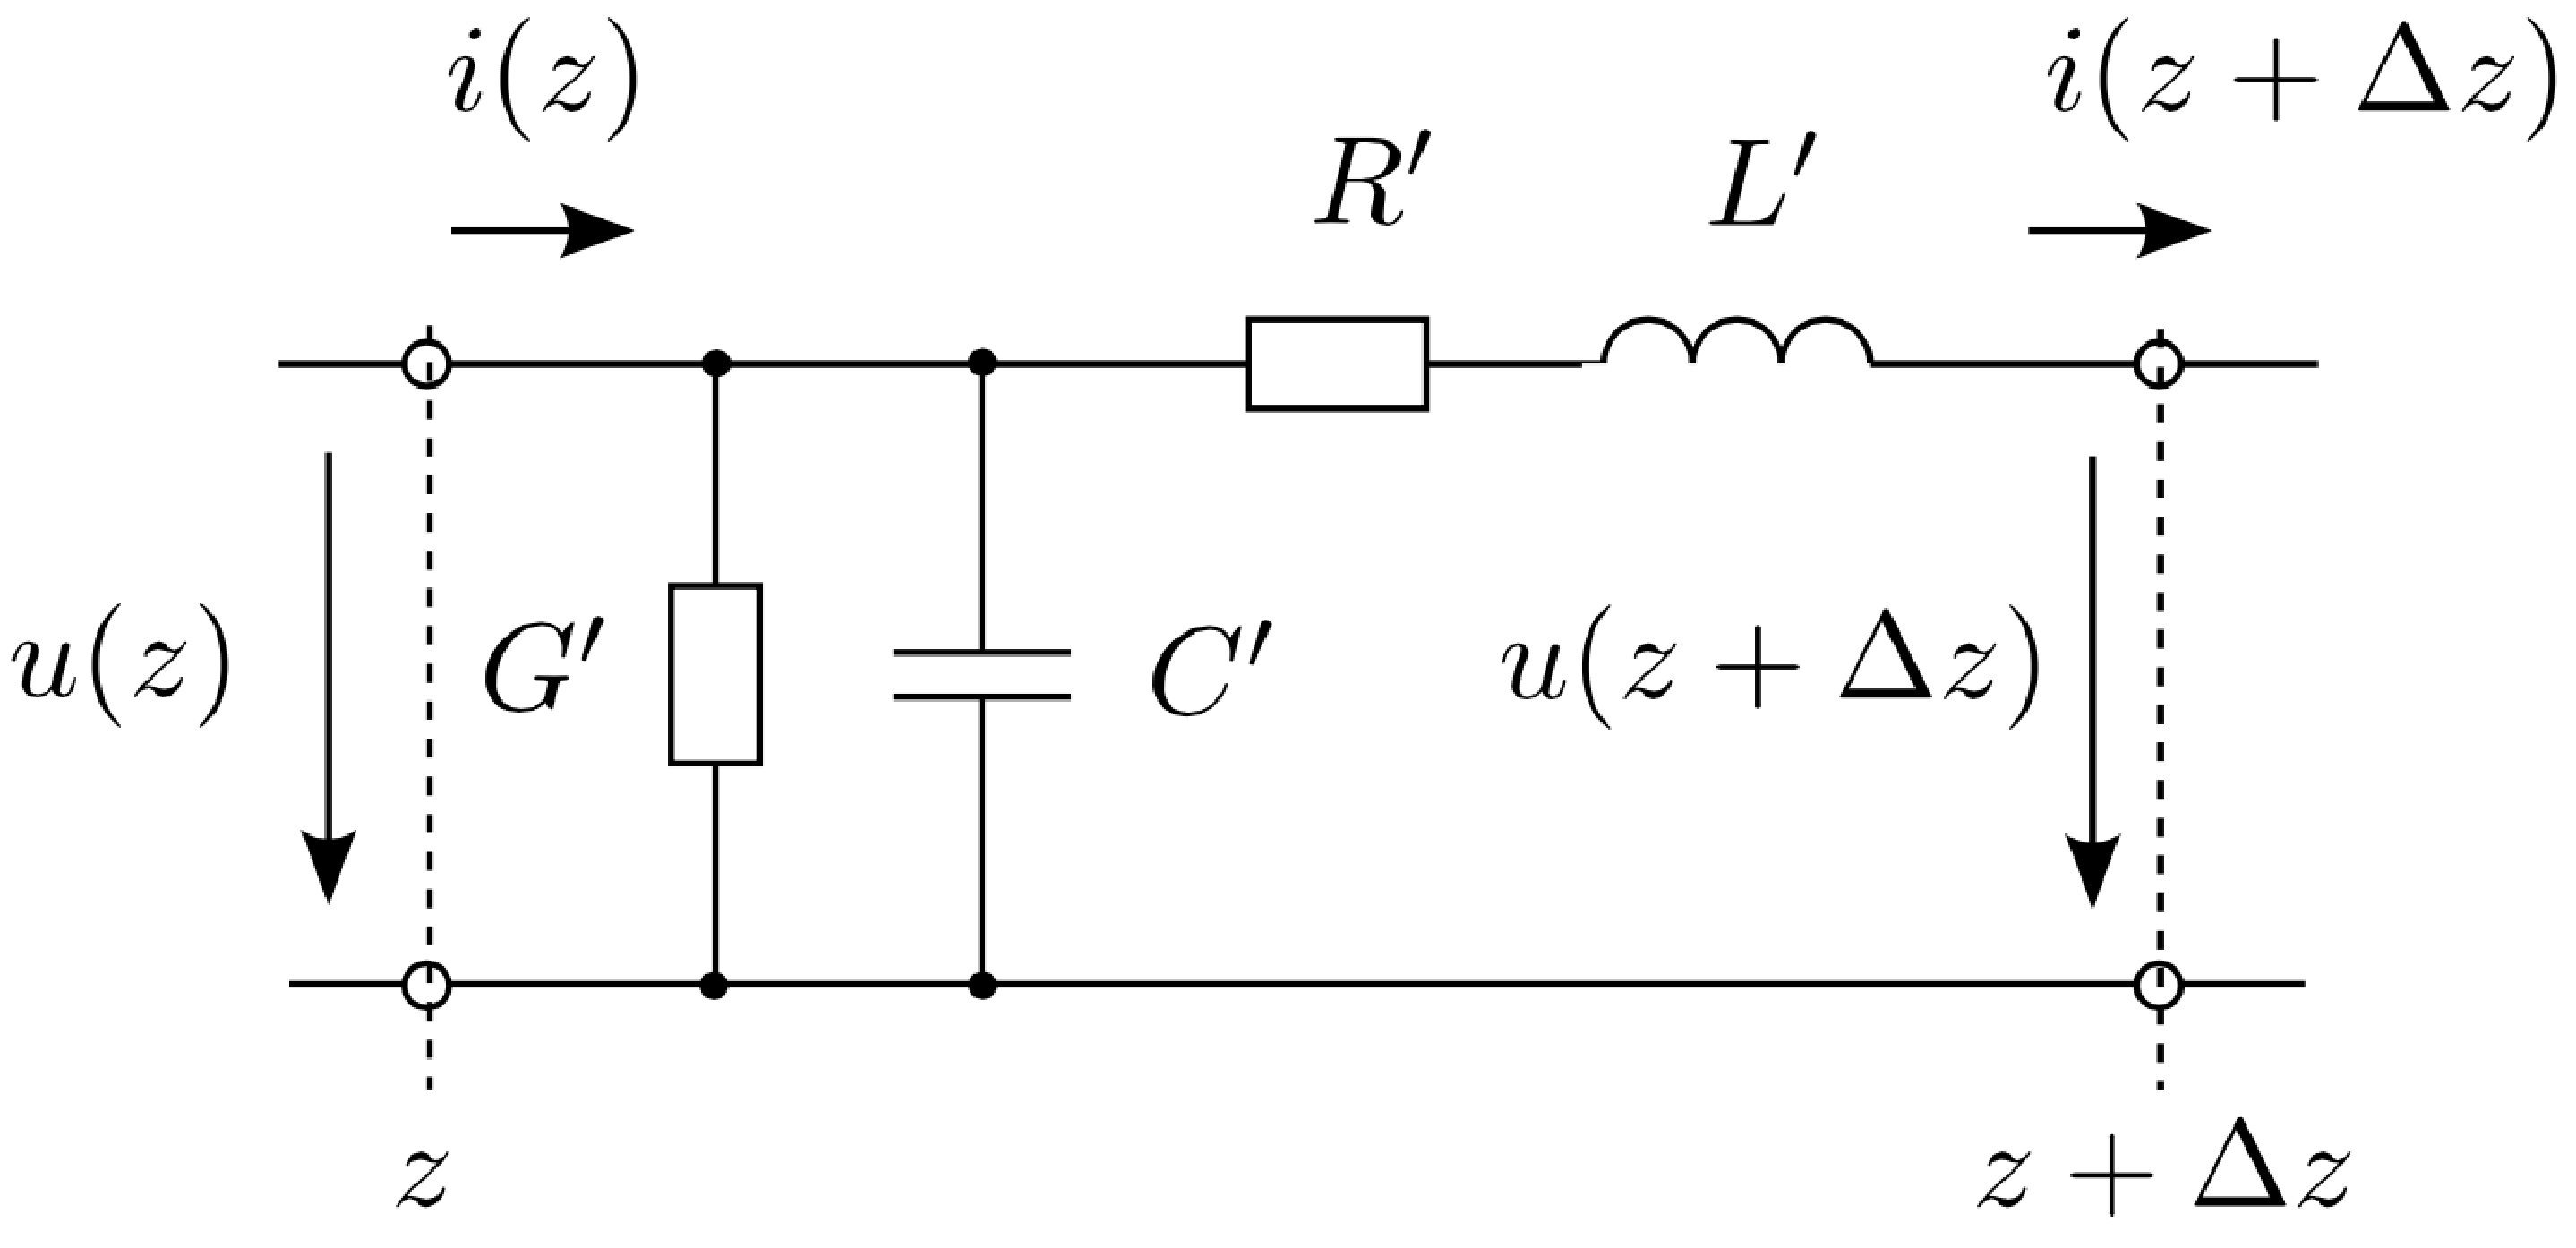
\includegraphics[width=11cm]{content/bilder/Leiterstueck.pdf}%
	\caption{Ersatzschaltbild eines elementaren Leiterstücks}
	\label{fig:ESBLeiterstueck}
\end{figure}

Bei einer längshomogenen Leitung darf die Annahme getroffen werden, dass die Induktivität $\Delta L$ und die Kapazität $\Delta C$ gleichförmig über die Länge $\Delta z$ verteilt sind. Man kann sie daher im Modell als Leiterbeläge ausdrücken. Die Gleichung \ref{eq:InduktiverLeitungsbelag} gibt den induktiven Leitbelag an. Die Gleichung \ref{eq:KapazitiverLeitungsbelag} zeigt den kapazitiven Leitbelag.
\begin{equation}
L'=\dfrac{\Delta L}{\Delta z}\label{eq:InduktiverLeitungsbelag}
\end{equation}
\begin{equation}
C'=\dfrac{\Delta C}{\Delta z}\label{eq:KapazitiverLeitungsbelag}
\end{equation}

Werden zudem die ohmschen Verluste im Leiter und allfällige dielektrische Verluste in der Isolation als Wirkwiderstände dargestellt, so lässt sich das Ersatzschaltbild einer Leitung gemäss Abbildung \ref{fig:ESBLeiterstueck} modellieren.
Für die Gleichungen \ref{eq:InduktiverLeitungsbelag}, \ref{eq:KapazitiverLeitungsbelag} und die Abbildung \ref{fig:ESBLeiterstueck} gilt:
\begin{enumerate}[leftmargin=2cm]
   \item[] $R'$: Ohmsche Leiterverlust/m [$\Omega/m$] 
   \item[] $L'$: Serie Induktivität/m  [$H/m$] 
   \item[] $G'$: Dielektrische Verluste/m  [$S/m$] 
   \item[] $C'$: Kapazität zwischen den Leiten/m  [$F/m$] 
   \item[] $\Delta m$: Abschnittslänge  [$m$] 
\end{enumerate} 
\todo{serieeninduktivität}
Die Spannung und der Strom auf einer Leitung kann als Summe von zwei Wellen beschrieben werden. Die eine Welle läuft vorwärts entlang der positiven $z$ Ausrichtung. Die rückwärts laufende Welle geht entlang der negativen z Achse. Der Strom und die Spannung können mit Hilfe der elementaren Leiterabschnitte $\Delta z$ an jedem Punkt $z$  der Leitung berechnet werden. Die Gleichung \ref{eq:UvonZundT} gibt die Summe der vor- und zurücklaufenden Spannungswellen an. Der Strom an jedem beliebigen Punkt auf der Leitung kann mit der Gleichung \ref{eq:IvonZundT} berechnet werden \cite{Tekom}.
\begin{eqnarray}\label{eq:UvonZundT}
U(z,t) &=& U_{v}e^{-\alpha z}e^{j(\omega t -\beta z)}+U_{r}e^{\alpha z}e^{j(\omega t \beta z)}
\end{eqnarray}
\begin{eqnarray}\label{eq:IvonZundT}
I(z,t) &=& I_{v}e^{-\alpha z}e^{j(\omega t -\beta z)}+I_{r}e^{\alpha z}e^{j(\omega t \beta z)}
\end{eqnarray}

\subsection{Anpassung und Reflexionen}
Die Anpassung ist nicht nur in Hochfrequenztechnik HF ein viel diskutiertes Thema, auch in der Gleichstromtechnik wird von Anpassung gesprochen. Es gibt verschiedene Formen der Anpassung. Zum Beispiel wird von Leistungsanpassung gesprochen, wenn möglichst viel Leitung einer Quelle einem Lastwiderstand zugeführt werden soll. Um das zu erreichen muss der Innenwiederstand  $R_i$ einer Quelle dem Lastwiderstand $R_L$ entsprechen.  Ein ganz anderes Ziel verfolgt die Wellenanpassung. Sie kommt immer dann zum Zuge, wenn auf einem Signalpfad die Signalreflexionen an den Übergängen des Mediums verhindert werden.
Man vergleicht immer die Eingangsimpedanz mit der Ausgangsimpedanz. Es ist  von $Z_{ein}$ und $Z_{aus}$ die Rede.
In diesem Kapitel werden zwei Arten der Anpassung genauer betrachtet. Es sind dies die:
\begin{itemize}
\item Leistungsanpassung
\item Wellenanpassung
\end{itemize}
Die Leistungsanpassung wird angewendet, wenn die maximale Leistungsübertragung gefordert ist. Die maximale Leistung in der Last wird erreicht, wenn der Lastwiderstand dem Quellenwiderstand entspricht. Bei rein ohmischen Quellen und Lastwiderstand bedeutet das:\\
\[R_{Quelle} = R_{Last}\]

Die Wellenanpassung wird auch Leitungsanpassung oder Impedanzanpassung genannt. Wellenanpassung ist in der Hochfrequenztechnik immer dann gefragt, wenn die zu übertragenden Wellen oder Impulse ohne Reflexionen von einer Quelle zu einer Last übertragen werden. Haben die Impedanzen der Quelle, der Leitung und der Last nur reelle Anteile, wird sowohl Wellenanpassung als auch Leistungsanpassung erreicht. Treten jedoch Impedanzen mit positivem oder negativem Imaginärteil auf, so muss für die Wellenanpassung das folgende Kriterium erfüllt sein: \\
\begin{eqnarray}\label{eq:ZeinZaus}
Z_{ein} = Z_{aus} = R_{ein} +jX_{ein} = R_{aus} + jX_{aus}
\end{eqnarray}

Im diesem Zusammenhang soll auch erwähnt sein, dass es auch die Spannungsanpassung und die Stromanpassung gibt, beides wird im Rahmen dieser Arbeit nicht erläutert. \\

Die Reflexionen und die Anpassung soll anhand eines Beispiels einer Leitung mit Abschlusswiderstand genauer näher erläutert werden. \\

Eine Quelle treibt eine vorwärtslaufende Welle in einer Leitung. Die Leitung besitzt einen Leitungswiderstand $Z_0$.  Das Ende der Leitung ist mit einem Abschlusswiderstand versehen. Dieser Widerstand stellt eine Lastimpedanz $Z_L$ zwischen dem Hin- und Rückleiter dar. \\
Man spricht von einer mit einer Lastimpedanz $Z_0$ abgeschlossenen Übertragungsleitung. Leitungsimpedanz $Z_0$ entspricht nicht exakt der Leitungsimpedanz $Z_L$, daher kommt es zu einer   Teilreflexion der vorlaufenden Welle. Das Verhältnis zwischen den Amplituden der rücklaufenden Welle und der vorlaufenden Welle wird als Reflexionskoeffizient r bezeichnet. \\

Reflexionskoeffizient r

\begin{eqnarray}\label{eq:Reflexionskoeffizient}
r=\dfrac{U_{R}}{U_{V}}=\dfrac{Z_{L}-Z_{V}}{Z_{L} + Z_{V}}=-\dfrac{I_{R}}{I_{V}}
\end{eqnarray}

%%%%%%%%%%%%%%%%%%%%%%%%%%%%%%%%%%%%%%%%%%%%%%%%%%%%%%%%%%%%%%%%%%%
\begin{figure}[!h]
	\centering
	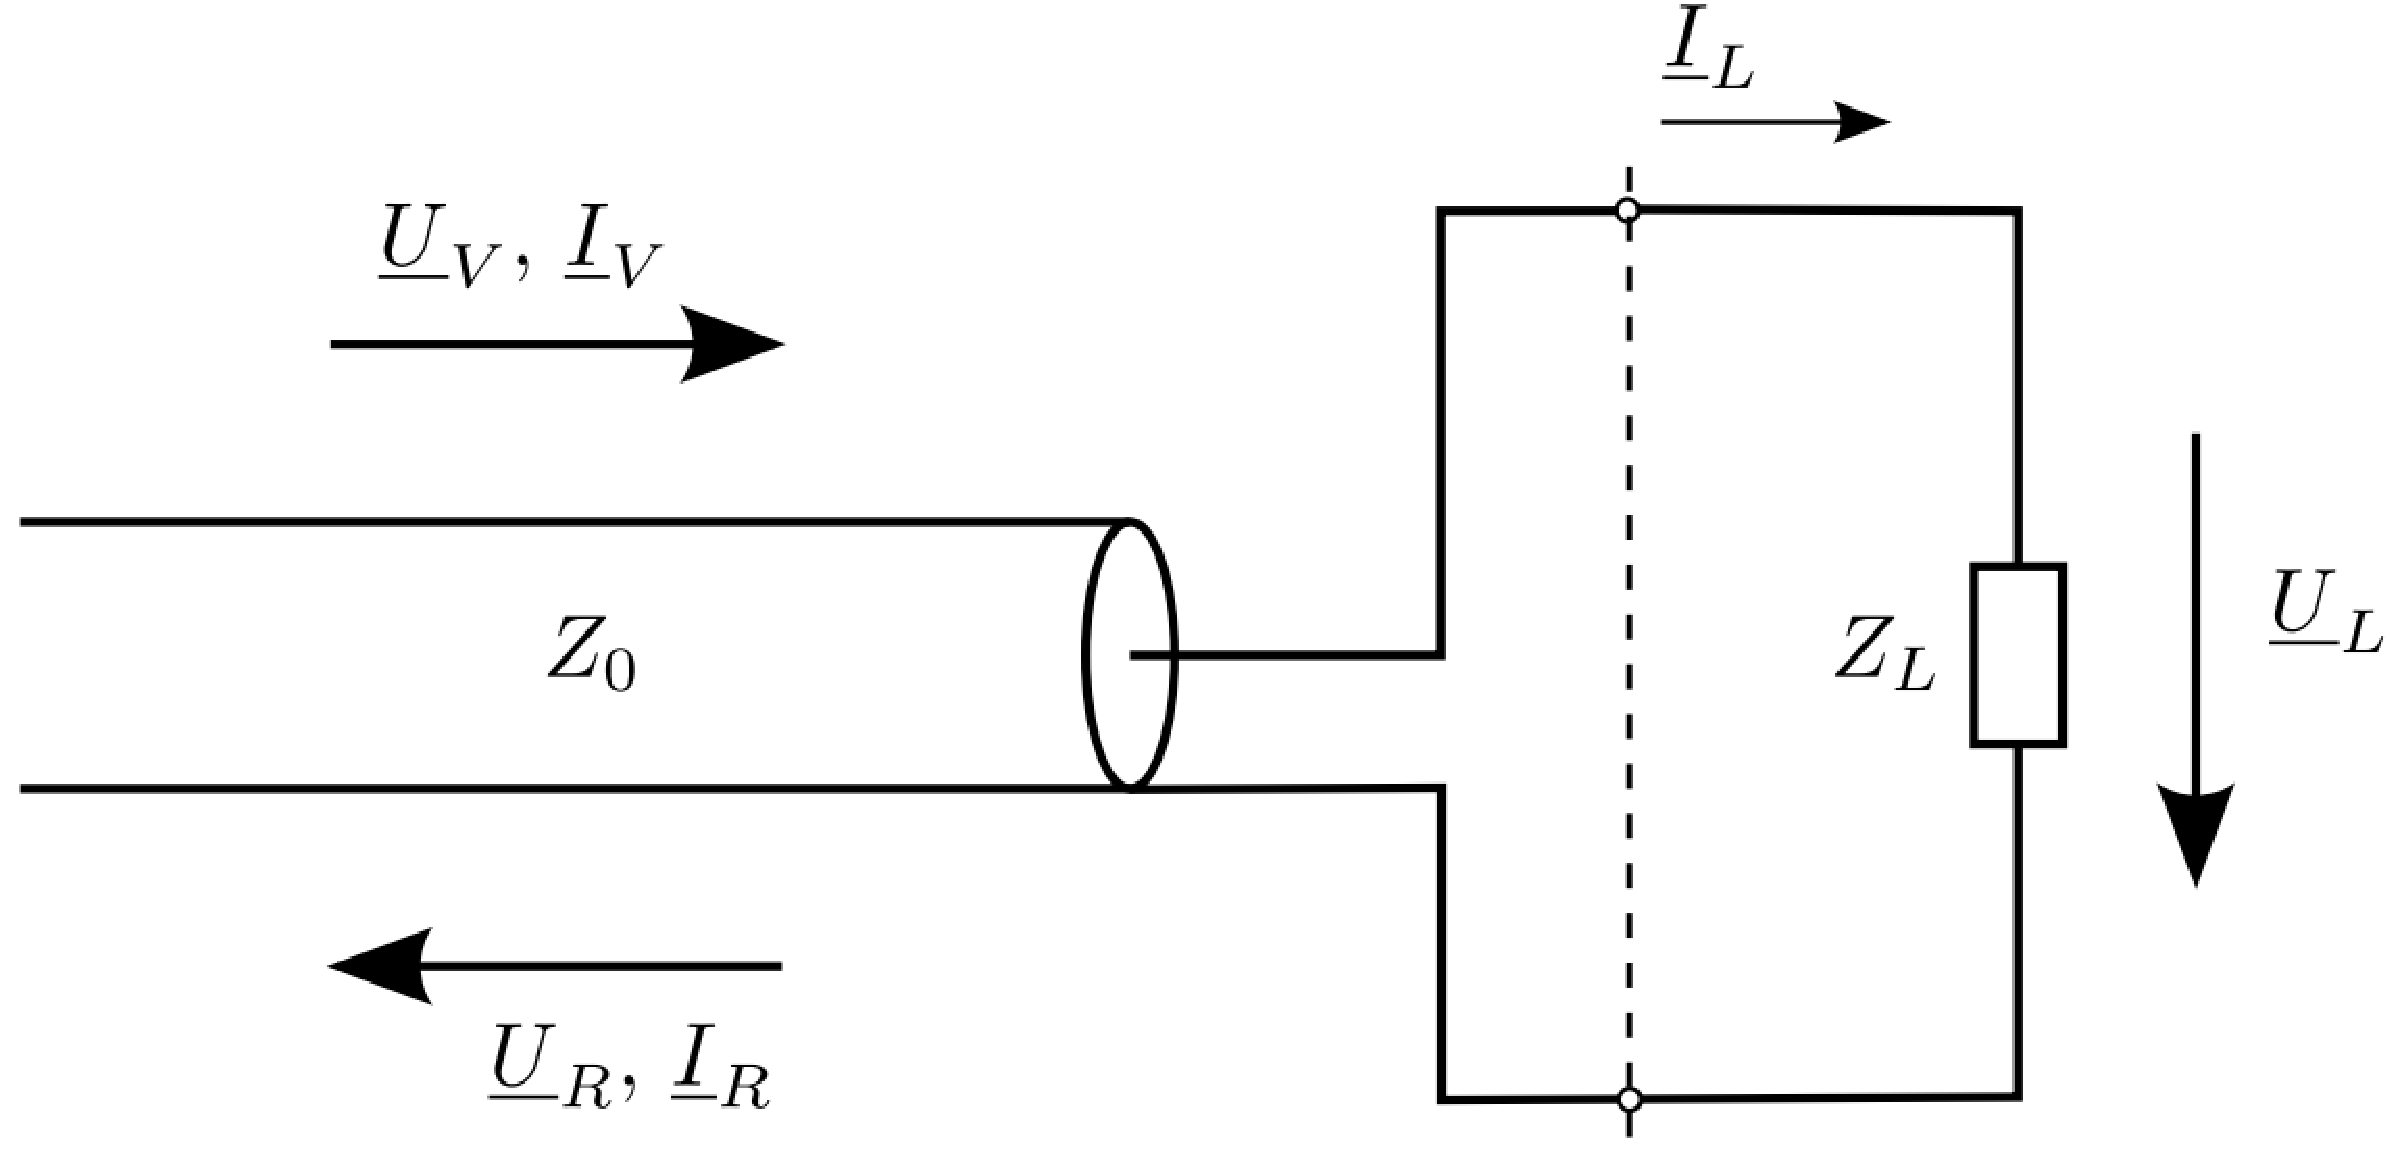
\includegraphics[width=10cm]{content/bilder/ReflexionenLeitungLastimpedanz.pdf}%
	\caption{Refelxionen einer Leitung an einer Lastimpedanz \cite{Tekom}}
	\label{FitzDipol}
\end{figure}
%%%%%%%%%%%%%%%%%%%%%%%%%%%%%%%%%%%%%%%%%%%%%%%%%%%%%%%%%%%%%%%%%%%


Die Spannung $U_L$ über der Last ergibt sich  aus der Überlagerung der vorlaufenden Spannungswelle und  rücklaufenden Spannugswelle. Dies ist in der Gleichung \ref{eq:AnpassungULast} gezeigt. In Gleichung \ref{eq:AnpassungILast} ist der Strom in der Last ersichtlich. Dieser wird aus der Vorlaufenden- und Rücklaufendenstromwelle gebildet.
\todo{Spannugswellen}

\begin{eqnarray}\label{eq:AnpassungULast}
U_L = U_V + U_R
\end{eqnarray}

\begin{eqnarray}\label{eq:AnpassungILast}
I_L = I_V + I_R
\end{eqnarray}

Durch die Überlagerung des vorlaufenden und rücklaufenden Signals gibt es eine Überlagerungskurve die örtlich konstante Maxima $U_{max}$ und Minima $U_{min}$ aufweist. Dies wird als stehende Welle bezeichnet. Dadurch kann die Spannung an den Knotenpunkten Werte zwischen Null und dem doppelten Wert der Spannung des vorlaufenden Signals aufweisen. An den Knotenpunkten heben sich die Wellen gegenseitig auf. Ihr Wert ist somit Null. Für die Beschreibung der Fehlanpassung haben sich neben dem Reflexionskoeffizient  $r$ noch weitere Begriffe etabliert: \\

Rückflussdämpfung $a$:\\
Die Rückflussdämpfung a wird in der englischen Literatur \textit{Return Loss} genannt.
\begin{eqnarray}\label{eq:Ruckflussdämpfung_a}
a=20\log\left(\left| \dfrac{U_V}{U_R}\right| \right)=-20\log(|r|)
\end{eqnarray}
Die Ruckflussdämpfung beschreibt als logarithmisches Mass, wie stark das rücklaufende Signal gegenüber dem vorlaufenden Signal gedämpft ist \cite{Tekom}.\\

Welligkeitsfaktor $s$:
\begin{eqnarray}\label{eq:Welligkeitsfaktor_s}
s=\dfrac{U_{max}}{U_{min}}=\dfrac{1+|r|}{1-|r|}
\end{eqnarray}
Der Welligkeitsfaktor $s$ \ref{eq:Welligkeitsfaktor_s} bezeichnet die Verhältnisse der Beträge von Maxima und Minima der stehenden Welle auf der Leitung. Der Welligkeitsfaktor $s$ wird in der englischen Literatur auch als \textit{Voltage Standing Wave Ratio} kurz VSWR bezeichnet. \\
\todo{Betrag Welligkeisfaktor s}

Anpassnetzwerke: \\
Nachrichtentechnische Systeme können als eine Kette von aktiven oder passiven Eintor- und Zweitorschaltungen dargestellt werden. Das heisst Quelle, Leitungen, Übergänge und Antennen werden als Zweitore betrachtet. Für eine einwandfreie Funktion bei der Zusammenschaltung der Übertragungskette muss der Lastwiderstand $Z_L$ zum Innenwiderstand $Z_I$ des Zweitors in einem bestimmten Verhältnis stehen. Die Eingangsimpedanz eines Zweitors wird oft als $Z_{ein}$ und die Ausgansimpedanz als $Z_{aus}$ bezeichnet. 
Um die Anpassungsbedingungen zu formulieren kann das Zweitor als eine Spannungsquelle mit dem Innenwiderstand $Z_I$ verstanden werden. Diese wird  durch den Lastwiderstand $Z_L$ belastet.

Leistungsanpassung: \\
Für die Übertragung der maximalen Wirkleistung von der Quelle zur Last  wird Leistungsanpassung benötigt. Um diese Bedingung zu erfüllen muss gelten:

\[Z_{ein} = Z_{aus}^*\]
Das bedeutet, eine induktive Komponente beim Innenwiderstand muss somit durch eine gleich grosse kapazitive Komponente beim Aussenwiderstand kompensiert werden und umgekehrt. Gleichzeitig müssen die beiden Wirkwiderstände gleiche Werte aufweisen. Das heisst, der Realteil von $Z_{ein}$ und $Z_{aus}$ sind gleich, jedoch sind die Imaginäranteile konjugiert komplex. Das bedeutet, dass die Blindwiderstände von Quelle und Last sich ausgleichen müssen. Dies geschieht, wenn eine ohmisch induktive Quelle durch eine ohmisch kapazitive Last kompensiert wird um das Leistungsanpassungskriterium zu erfüllen. \\

Wellenanpassung: \\
Bei der Leistungsanpassung kommt es auf Grund der unterschiedlichen Blindwiderstände zu eine Stossstelle für das zu übertragende Signal. Dies führt zu Reflexionen, dabbei wird  ein Teil des Signals reflektiert. Stehende Wellen sind das Resultat. Um diese störenden Einflüsse zu vermeiden, muss für komplexe Widerstände folgende Beziehung erfüllt sein:
\[Z_{I} = Z_{L}\]

Diese Anpassung bezeichnet man als Impedanzanpassung oder Leitungsanpassung. Die bisherigen Erkenntnisse zeigen, dass nur im Falle rein reeller Werte für den Innen- und den  Lastwiderstand, das heisst wenn $X_i = X_L = 0$ sind, Leistungsanpassung und Wellenanpassung identisch sind. Für den allgemein gültigen Fall komplexer Widerstände ist stets eine Entscheidung zwischen Übertragung maximaler Wirkleistung,  mit Inkaufnahme von Teilreflexionen auf den Leitungen oder einer reflexionsfreien Übertragung mit einem Leitungswirkungsgrad von $\eta <50 \%$ zu treffen. In der Nachrichtentechnik bezieht man sich in der Regel auf die Wellenanpassung. Die bei der Leistungsanpassung entstehenden Reflexionen  sind störender als die Verluste durch die Übertragung geringerer Wirkleistung. Die bei der Wellenanpassung resultiert. Nur bei Leistungsverstärkern, zum Beispiel in Endstufe eines Senders, spielt die Leistungsanpassung eine nicht zu vernachlässigende Rolle. Für eine optimale Leistungsübertragung ist es notwendig, dass spezielle Anpassnetzwerke verwendet werden. \\

Die maximale Wirkleistung wird in einem Gleichstromkreis bei $R_Q = R_L$ abgegeben. Es besteht Leistungsanpassung. Das heisst, die in dem $R_L$ umgesetzte Leistung ist maximal. Der Wirkungsgrad $\eta$ entspricht $50\%$, da dieselbe Leistung wie in der Last im Innenwiderstand der Quelle $R_Q$ umgesetzt wird. Die Formel \ref{eq:PmaxLeistungsanpassung} zeigt die maximale Leistung in der Last. Die Abbildung \ref{fig:LeistungsanpassungU0_RQ_RL} zeigt eine Schaltung, bei der die Bedingung für Leistungsanpassung $R_Q = R_L$ gilt.
\begin{eqnarray}\label{eq:PmaxLeistungsanpassung}
P_{Last_{max}}=\dfrac{U_{0}^2}{4R_Q} bei R_Q=R_L
\end{eqnarray}

\begin{figure}[h]
	\begin{center}
	\begin{tikzpicture}
	\draw[line width=1.5pt](3, 3.5) circle (0.5) node at (3,3.5) {$U_{0}$};%Quelle
	\draw[line width=1.5pt] (3, 5) -- (4.5, 5);%oben kurz

	\draw[line width=1.5pt] (3, 2) -- (3, 3);%von unten zur Quelle
	\draw[line width=1.5pt] (3, 4) -- (3, 5);%von der Quelle nach oben
	\draw[line width=1.5pt](4.5, 4.75) rectangle (5.5, 5.25) node at (5, 5.5) {$R_Q$};%RQ

	\draw[line width=1.5pt, -*](5.5, 5)  -- (7, 5);%oben bis zum Punkt
	\draw[line width=1.5pt, -*](3, 2)  -- (7, 2);%unten bis zum Punkt
	
	\draw[line width=1.5pt](7, 5)  -- (8.5, 5);%oben 
	\draw[line width=1.5pt](7, 2)  -- (8.5, 2);%unten 
	\draw[line width=1.5pt](8.5, 5)  -- (8.5, 4);%oben nach unten zu RL
	\draw[line width=1.5pt](8.5, 2)  -- (8.5, 3);%unten nach oben zu RL

 	\draw[line width=1.5pt](8.25, 3) rectangle (8.75, 4) node at (9.25, 3.5) {$R_L$} ;%RL
 	\draw[line width=1.5pt, ->, >=latex](6.5, 3.5) -- (7.5, 3.5) node at (7, 3.8) {$P_a$};

	\end{tikzpicture}
	\end{center}
\caption{Leistungsanpassung mit $R_Q = R_L$}
\label{fig:LeistungsanpassungU0_RQ_RL}
\end{figure}


Bei Wechselgrössen kann ein Transformator für die Leistungsanpassung eingesetzt werden. Ist der Quellenwiderstand $R_Q$ oder der Lastwiderstand $R_L$  reaktiv, das heisst induktiv oder kapazitiv, dann sind die Schaltungen stark frequenzabhängig. So besitzt beispielsweise eine Antenne nur bei einer bestimmten Frequenz einen rein reellen Innenwiderstand $R_i$. Bei allen andern Frequenzen sind sowohl Real- als auch Imaginärteil vorhanden. Eine Möglichkeit für eine Korrektur ist in der Abbildung \ref{AnpassungKomplexerLast} dargestellt. Auch diese  Anpassung ist frequenzabhängig und nur für die Entwurfsfrequenz optimal, aber dank der Transformation ist Leitungsanpassung möglich.
\todo{Bild selber zeichnen}
%%%%%%%%%%%%%%%%%%%%%%%%%%%%%%%%%%%%%%%%%%%%%%%%%%%%%%%%%%%%%%%%%%%
\begin{figure}[!h]
	\centering
	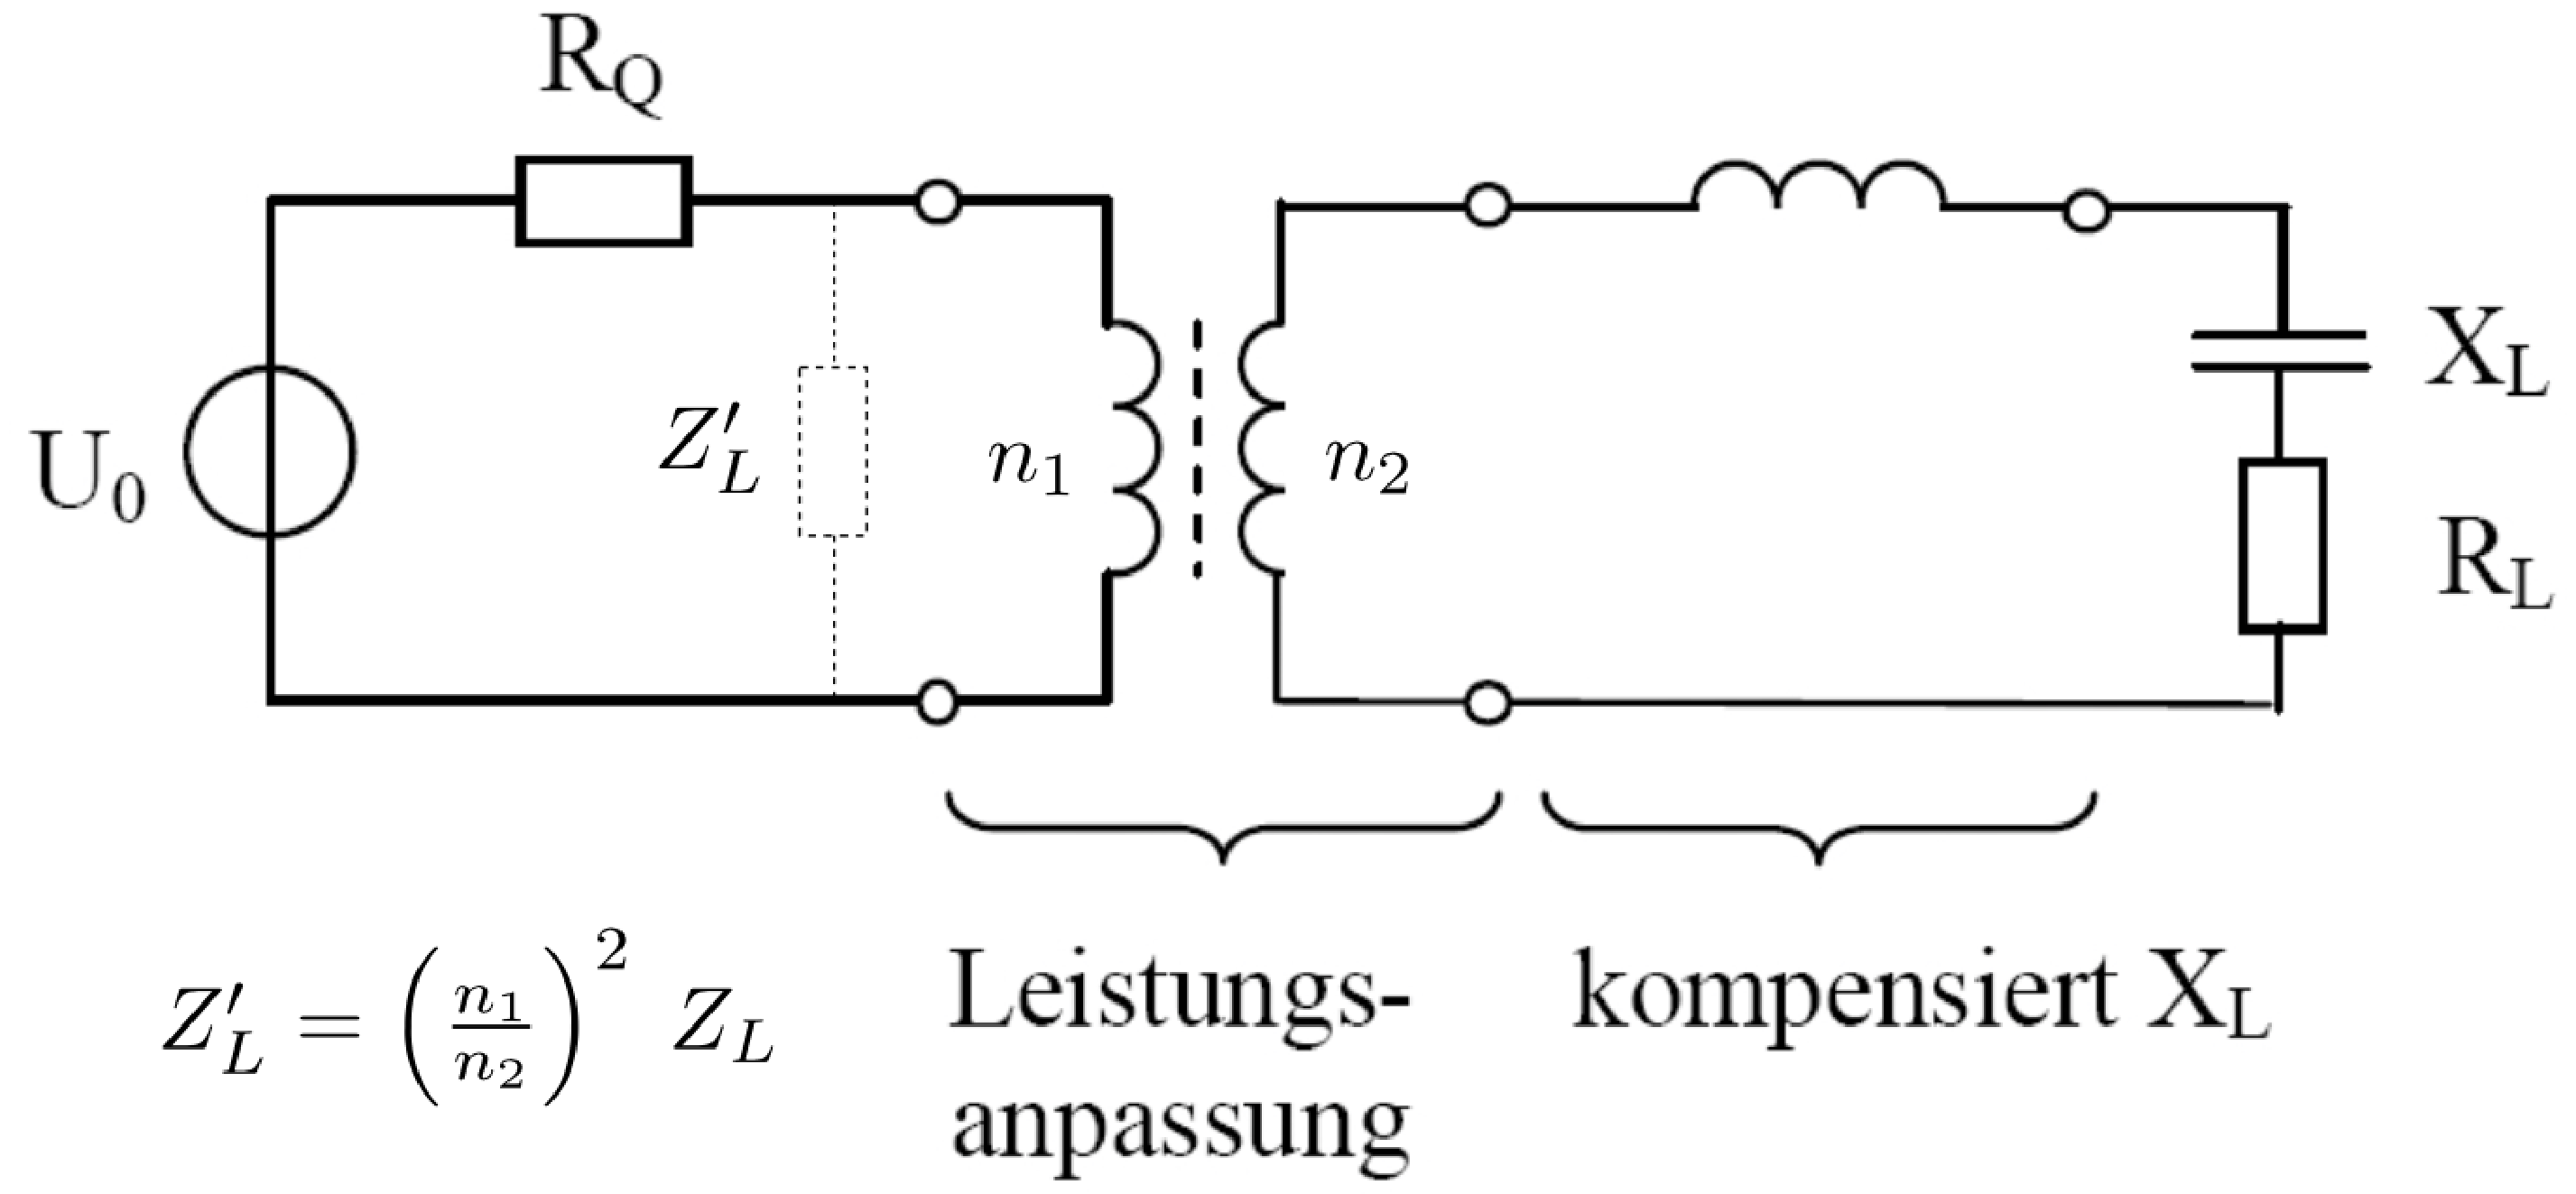
\includegraphics[width=10cm]{content/bilder/AnpassungKomplexerLast.pdf}%
	\caption{leitungsanpassung für eine komplexe Last \cite{Tekom}}
	\label{AnpassungKomplexerLast}
\end{figure}
%%%%%%%%%%%%%%%%%%%%%%%%%%%%%%%%%%%%%%%%%%%%%%%%%%%%%%%%%%%%%%%%%%%

\textbf{Entwurf eines Ohm’schen Anpassnetzwerkes:} \\
Für die Anpassung einer Generatorimpedanz $R_Q$, welche grösser ist als die Last $R_L$, kann die Schaltung von Abbildung \ref{fig:Leistungsanpassung_RQ_grösser_als_RL} verwendet werden. Die Widerstände R1 und R2 berechnen sich nach folgenden Beziehungen der Gleichung \ref{eq:R1R2wennRQgrösserRL}:

\begin{align}\label{eq:R1R2wennRQgrösserRL}
R1 &= \sqrt{RQ(RQ-RL)}\\
R2 &= \dfrac{RQ RL}{R1}\\
a_{dB} &= 20\log \left( \sqrt{\dfrac{RQ}{RL}}+\sqrt{\dfrac{RQ}{RL}-1}\right)
\end{align}

\begin{figure}[h]
	\begin{center}
	\begin{tikzpicture}
%	\draw[line width=1.5pt](3, 3.5) circle (0.5) node at (3,3.5) {$U_{0}$};%Quelle
%	\draw[line width=1.5pt] (3, 5) -- (4.5, 5);%oben kurz

%	\draw[line width=1.5pt] (3, 2) -- (3, 3);%von unten zur Quelle
	\draw[line width=1.5pt, *-] (1, 5) -- (3, 5);%oben zu R1
	\draw[line width=1.5pt](3, 4.75) rectangle (4, 5.25) node at (3.5, 5.5) {$R1$};%R1

	\draw[line width=1.5pt, *-](5, 5.1)  -- (5, 4);%oben nach unten zu RL
	\draw[line width=1.5pt, *-](5, 1.9)  -- (5, 3);%unten nach oben zu RL
 	\draw[line width=1.5pt](4.75, 3) rectangle (5.25, 4) node at (5.6, 3.5) {R2};%R2

	\draw[line width=1.5pt, -*](4, 5)  -- (7, 5);%oben bis zum Punkt
	\draw[line width=1.5pt, *-*](1, 2)  -- (7, 2);%unten bis zum Punkt
	
	\draw[line width=1.5pt](5, 5)  -- (8.5, 5);%oben 
	\draw[line width=1.5pt](7, 2)  -- (8.5, 2);%unten 
	\draw[line width=1.5pt](8.5, 5)  -- (8.5, 4);%oben nach unten zu RL
	\draw[line width=1.5pt](8.5, 2)  -- (8.5, 3);%unten nach oben zu RL

 	\draw[line width=1.5pt](8.25, 3) rectangle (8.75, 4) node at (9.25, 3.5) {$R_L$} ;%RL
 	\draw[line width=1.5pt, ->, >=latex](0, 3.5) -- (1.5, 3.5) node at (0.75, 4) {$Z_{ein}=RQ$};

	\draw[line width=1.5pt,style=dashed](2,1.5) rectangle (6, 6);
	\end{tikzpicture}
	\end{center}
\caption{Anpassung für $R_Q > R_L$}
\label{fig:Leistungsanpassung_RQ_grösser_als_RL}
\end{figure}

Gilt es eine hochohmige Last RL an eine Quelle mit einem RQ der kleiner ist als RL anzupassen, so können die Schaltung von Abbildung \ref{fig:LeistungsanpassungU0_RQkleiner_als_RL} und die mathematischen Beziehungen und den Gleichungen \ref{eq:R1R2wennRLgrösserRQ}  verwendet werden.

\begin{align}\label{eq:R1R2wennRLgrösserRQ}
R1 &= \sqrt{RL(RL-RQ)}\\
R2 &= \dfrac{RQ RL}{R1}\\
a_{dB} &= 20\log \left( \sqrt{\dfrac{RL}{RQ}}+\sqrt{\dfrac{RL}{RQ}-1}\right)
\end{align}
\begin{figure}[h]
	\begin{center}
	\begin{tikzpicture}

	\draw[line width=1.5pt, *-] (1, 5) -- (4, 5);%oben zu R1
	\draw[line width=1.5pt](4, 4.75) rectangle (5, 5.25) node at (4.5, 5.5) {$R1$};%R1

	\draw[line width=1.5pt, *-](3.5, 5.1)  -- (3.5, 4);%oben nach unten zu RL
	\draw[line width=1.5pt, *-](3.5, 1.9)  -- (3.5, 3);%unten nach oben zu RL
 	\draw[line width=1.5pt](3.25, 3) rectangle (3.75, 4) node at (4, 3.5) {R2};%R2

	\draw[line width=1.5pt, -*](5, 5)  -- (7, 5);%oben bis zum Punkt
	\draw[line width=1.5pt, *-*](1, 2)  -- (7, 2);%unten bis zum Punkt
	
	\draw[line width=1.5pt](7, 5)  -- (8.5, 5);%oben von R1 zum Punkt 
	\draw[line width=1.5pt](7, 2)  -- (8.5, 2);%unten 
	\draw[line width=1.5pt](8.5, 5)  -- (8.5, 4);%oben nach unten zu RL
	\draw[line width=1.5pt](8.5, 2)  -- (8.5, 3);%unten nach oben zu RL

 	\draw[line width=1.5pt](8.25, 3) rectangle (8.75, 4) node at (9.25, 3.5) {$R_L$} ;%RL
 	\draw[line width=1.5pt, ->, >=latex](0, 3.5) -- (1.5, 3.5) node at (0.75, 4) {$Z_{ein}=RQ$};

	\draw[line width=1.5pt,style=dashed](2,1.5) rectangle (6, 6);
	\end{tikzpicture}
	\end{center}
\caption{Anpassung für $R_Q < R_L$}
\label{fig:LeistungsanpassungU0_RQkleiner_als_RL}
\end{figure}

\textbf{Entwurf eines verlustfreien L-Netzwerkes}\\
Ein einfaches, verlustfreies Anpassnetzwerk besteht aus zwei Reaktanzen. Der Entwurfsansatz besteht darin, dass eine Reaktanz $X_{p}$ parallel zum grösseren Widerstand, in Abbildung xxxx wäre dies der Quellenwiderstand $R_{Q}$, geschalten wird. In diesem Fall folgt für die Impedanz $Z_{links} $von der Trennlinie... \\
\todo{Bild einfügen L Netzwetzwerk}
Formel\\
\todo{Formel 2.39}
$X_p$  kann nun so gewählt werden, dass der Realteil von $Z_{Links}$  dem Lastwiderstand $R_L$ entspricht. \\
\begin{equation}
R_{Links}= R_L
\end{equation}
Als nächstes gilt es, die so eingeführte imaginäre Grössse $X_{Links}$ auf der rechten Seite der 
Trennlinie zu kompensieren, indem die Seriereaktanz $X_{s}$entsprechend gewählt wird: 
\begin{equation}
X_{Links}= -jX_s
\end{equation}
Als letzten Schritt gilt es die Werte für die Induktivität $L$ und Kapazität $C$ für die gewünschte Frequenz zu berechnen. 
\begin{equation}
jX_{L}= j\omega L und jX_c=\dfrac{-j}{\omega C}
\end{equation}




%%%%%%%%%%%%%%%%%%%%%%%%%%%%%%%%%%%%%%%%%%%%%%%%%%%%%%%%%%%%%%%%%%%%%%%%%%%%%%%%%%%%%%%%%%%%%%%%%%%%%%%%%%%%%%%%%%%%
\subsection{Speisung}
\todo{Speisung und Anpassung auseinanderhalten}
Unter der Speisung der Antenne wird die Leistungszuführung verstanden. Damit eine Antenne strahlt, muss diese mit einer Spannungswelle angeregt werden. Die Strom und Spannungsverteilung der Antenne ist für das Abstrahlverhalten verantwortlich. 


\begin{itemize}
\item 	Leistungsanpassung
\item 	Singalanpassung
\end{itemize}
Leistungsanpassung wird benötigt, wenn der Leistungsfluss möglichst unbeeinträchtigt sein soll. Es muss gelten
$Z_{ein}=Z_{aus}*$.
Das bedeutet, dass der Realanteil von $Z_{ein}$ und $Z_{aus}$ gleich ist jedoch der Imaginärteil von $Z_{aus}$ muss den konjugiert komplexen Wert des $Z_{ein}$ aufweisen. Mit anderen Worten, $Z_{aus}$ hat beim Imaginärteil ein umgekehrtes Vorzeichen als der $Z_{ein}$. Leistungsanpassung kommt bei Leistungsendstufen oder allgemein dort zur Anwendung, wo es besonders wichtig ist, dass möglichst viel der erzeugten Leistung von der Last aufgenommen wird. Man bedenke, das ist im besten Falle nie mehr als 50\%.
Signalanpassung wird angewendet, wenn möglichst keine Reflexionen auf der Leitung entstehen sollen. Es muss gelten:\\
$Z_{ein}=Z_{aus}$\\%zentrieren
Die Signalanpassung ist dann gewünscht, wenn die Qualität des Signals Vorrang hat und keinerlei Reflexionen erwünscht sind. In diesem Fall ist das Stehwellenverhältnis SWR = 1.
Um die jeweilig gewünschte Anpassung zu erreichen kommen Anpassnetzwerke zum Einsatz. Diese sind meist passive Netzwerke mit Induktivitäten L und Kapazitäten C. Manchmal kommt zur Kapazität und zur Induktivität ein Widerstand hinzu.\\
Ein Beispiel für Anpassung.\\
Eine Quelle mit einem Ausgangswiderstand von nicht 50 Ohm reell wird mit Hilfe einer ersten Anpassung auf eine 50 Ohm Leitung angepasst. Am Ende der 50 Ohm Leitung wird ein weiteres Anpassungsnetzwerk benötigt. Damit wird die Leitung und die Antennen aufeinander abgestimmt.\\


%%%%%%%%%%%%%%%%%%%%%%%%%%%%%%%%%%%%%%%%%%%%%%%%%%%%%%%%%%%%%%%%%%%
\begin{figure}[!htb]
	\centering
	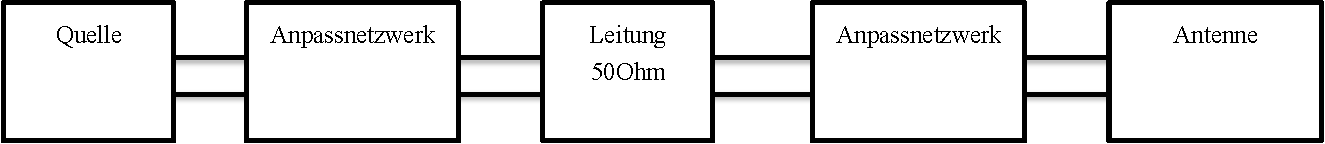
\includegraphics[width=8cm]{content/bilder/Anpassung.pdf}%
	\caption{Blockschaltbild einer Anpassung von der Quelle zur Antenne}
	\label{Anpassung}
\end{figure}
%%%%%%%%%%%%%%%%%%%%%%%%%%%%%%%%%%%%%%%%%%%%%%%%%%%%%%%%%%%%%%%%%%%
\todo{Bild Anpassung selber machn}

Wenn eine 50 Ohm Leitung an eine Antenne angeschlossen wird,  wird oft ein Anpassnetzwerk zwischen der Leitung und der Antenne benötigt.  Antennen haben einen  reellen Strahlungswiderstand $R_{rad}$. Je nach Typ einen kapazitiven oder einen induktiven Anteil.
%%%%%%%%%%%%%%%%%%%%%%%%%%%%%%%%%%%%%%%%%%%%%%%%%%%%%%%%%%%%%%%%%%%
\begin{figure}[!htb]
	\centering
	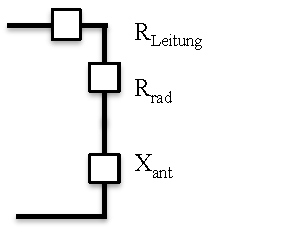
\includegraphics[width=5cm]{content/bilder/ESB_Antenne.pdf}%
	\caption{Ersatzschaltbild einer Antenne}
	\label{ESBantenne}
\end{figure}
%%%%%%%%%%%%%%%%%%%%%%%%%%%%%%%%%%%%%%%%%%%%%%%%%%%%%%%%%%%%%%%%%%%




%\begin{figure}
%\begin{center}
%\begin{circuitikz}
%\draw (1,1)--(3,1);
%\end{circuitikz}
%\end{center}
%\end{figure}
%%%%%%%%%%%%%
%%%%%%%%%%%%%%%%%%%%%%
%\begin{ circuitikz }[ scale =1.2]
%\begin{tikzpicture}
%\draw(0,0) node[anchor=east]{B} to [short, o-*] (1,0)
%to [R=20<\ohm>, *-*] (1,2)
%%to [R=10<\ohm>, v=$v_x$] (3,2) −− (4,2)
%%to [ cI=$\frac{\siemens}{5} v_x$, *−*] (4,0) −− (3,0)
%%to [R=5<\ohm>, *−*] (3,2)
%(3,0) −− (1,0)
%(1,2) to [short, −o] (0,2) node[anchor=east]{A};
%\end{tikzpicture}
%\end{ circuitikz }
%%%%%%%%%%%%%%%%%%%%%%

\begin{figure}[h]
	\begin{center}
	\begin{tikzpicture}
	\draw[line width=1.5pt](3, 3.5) circle (0.5) node at (3,3.5) {Uq};
	\draw[line width=1.5pt] (3, 5) -- (4.5, 5);
	%\draw[line width=1.5pt] (3, 2) -- (7, 2);
	\draw[line width=1.5pt, -*](3, 2)  -- (7, 2);
	\draw[line width=1.5pt] (3, 2) -- (3, 3);
	\draw[line width=1.5pt] (3, 4) -- (3, 5);
	\draw[line width=1.5pt](4.5, 4.75) rectangle (5.5, 5.25) node at (5, 5.5) {Rq} node at (5, 4.5) {50 Ohm};
	%\draw[line width=1.5pt] (5.5, 5) -- (7, 5);
	\draw[line width=1.5pt, -*](5.5, 5)  -- (7, 5);
	
	\draw[line width=1.5pt](7, 1.5) rectangle (12, 5.5) node at (9.5, 6) {Anpassungsnetzwerk};
	\draw[line width=1.5pt, *-](12, 5)  -- (13.5, 5);
	\draw[line width=1.5pt, *-](12, 2)  -- (16, 2);
	\draw[line width=1.5pt](13.5, 4.75) rectangle (14.5, 5.25) node at (14, 5.5) {$R_{v}$};
	\draw[line width=1.5pt](14.5, 5)  -- (16, 5);
	\draw[line width=1.5pt](16, 5)  -- (16, 4.4);
	\draw[line width=1.5pt](15.75, 3.4) rectangle (16.25, 4.4) node at (17, 3.9) {$R_{rad}$};%Rrad
	\draw[line width=1.5pt](16, 3.4)  -- (16, 2.8);
	\draw[line width=1.5pt](15.75, 2.8)  -- (16.25, 2.8);%Kondensator oben
	\draw[line width=1.5pt](15.75, 2.6)  -- (16.25, 2.6);%Kondensator unten
	\node at (17, 2.7) {$X_{ant}$};
	\draw[line width=1.5pt](16, 2.6)  -- (16, 2);
	
	\draw[line width=1.5pt, ->, >=latex](6.5, 4)  -- (8, 4) node at (8, 3.5) {$P_{ein}$};
	\draw[line width=1.5pt, ->, >=latex](11.5, 4)  -- (13, 4) node at (13, 3.5) {$P_{ant}$};
	
	\coordinate (A) at (7, 1);
	\coordinate (B) at (7, 0);
	\coordinate (a) at (10, 0.5);
	\draw[line width=1.5pt, cap=round,->](A) .. controls (a) .. (B) node at (6.5, 0.5) {S11} node at (5.5, 0.5) {$\Gamma$};
	\draw [-latex,line width=1.5pt](11.5,1) |-(13,2.5) node at (11.5, 0.5) {$Z_{ant}$};
	
	\node at (17.5, 6) {$\eta_{rad}=\dfrac{R_{rad}}{Rv+R_{rad}}$};
	\node at (9.5, 7) {$\eta_{overall}=\dfrac{P_{rad}}{P_{ein}}$};
	
	\node at (18, 2.7) {$\varepsilon$};
	\node at (18.5, 2.7) {$\delta$};
	
	\draw[->,line width=0.5pt,decorate, decoration=snake ](18, 4.1) -- (19.5, 4.6);
	\draw[->,line width=0.5pt, decorate, decoration=snake](18, 3.9) -- (19.5, 3.9);
	\draw[->,line width=0.5pt, decorate, decoration=snake](18, 3.7) -- (19.5, 3.1);
	\node at (20, 3.9) {$P_{rad}$};
	\end{tikzpicture}
	\end{center}
\caption{ESB einer Quelle mit Anpassnetzwerk  und einer Antenne}
\label{AnpassungQuelleAntenne}
\end{figure}

